
% \setchapterpreamble[ur]{%
% \dictum[I.~Berlin~\cite{berlin_blueskies}]{%
% Blue skies smilin' at me\\
% Nothin' but blue skies do I see}%
% \vspace*{2cm}}

% \setchapterpreamble[ur]{%
% \dictum[G.~R.~R.~Martin~\cite{martin1997game}]{%
% `It is known,' Irri agreed.}%
% \vspace*{2cm}}



%%%%%%%%%%%%%%%%%%%%%%%%%%%%%%%%%%%%%%%%%%%%%%%%%%%%%%%%%%%%
\chapter{An effective theory for Higgs physics}
\label{chapter:foundations}
%%%%%%%%%%%%%%%%%%%%%%%%%%%%%%%%%%%%%%%%%%%%%%%%%%%%%%%%%%%%

\firstword{I}{n this chapter} we review some of the essential concepts
that underlie the research presented in this thesis. First, we briefly
summarise the role of the Higgs boson in the Standard Model (SM) and
its phenomenology at the LHC.  \autoref{sec:foundations_eft} then
presents a pedagogical introduction to effective field theories
(EFTs). In \autoref{sec:foundations_higgs_eft} we combine these ideas
and construct an effective field theory for the Higgs sector.

Our introduction to Higgs physics is superficial, and the EFT part
eschews mathematical rigour in favour of a broad picture of the
central ideas. For a more thorough introduction to Higgs physics, see
for instance Reference~\cite{Plehn:2009nd}. For an extensive
introduction to EFTs, see References~\cite{Georgi:1994qn,
  Kaplan:2005es}. Note that \autoref{sec:foundations_eft} is largely
identical to Reference~\cite{Brehmer:EFTlecture}. Some of the examples
are taken from References~\cite{Georgi:1994qn, Kaplan:2005es}.



%%%%%%%%%%%%%%%%%%%%%%%%%%%%%%%%%%%%%%%%%%%%%%%%%%%%%%%%%%%%
\section{The Higgs boson at the LHC}
\label{sec:foundations_Higgs}
%%%%%%%%%%%%%%%%%%%%%%%%%%%%%%%%%%%%%%%%%%%%%%%%%%%%%%%%%%%%


%%%%%%%%%%%%%%%%%%%%%%%%%%%%%%%%%%%%%%%%%%%%%%%%%%%%%%%%%%%%
\subsection{The Standard Model Higgs sector}
%%%%%%%%%%%%%%%%%%%%%%%%%%%%%%%%%%%%%%%%%%%%%%%%%%%%%%%%%%%%

In the Standard Model, the Higgs boson is part of a scalar $SU(2)_L$
doublet $\phi$. The relevant terms in the Lagrangian are
%
\begin{multline}
  \lgr{SM} \supset (D_\mu \phi)^\dagger (D^\mu \phi) - \mu^2 \, \phisq - \lambda \, (\phisq)^2 \\
            - \sum_{\text{generations}} \left(    y_u \, {\twovec {\overbar u} {\overbar d}}_L \tilde \phi \, u_{R} 
                                                           + y_d \, {\twovec {\overbar u} {\overbar d}}_L \phi \, d_{R}
                                                           + y_\ell \, {\twovec {\overbar \nu} {\overbar \ell^-}}_L \phi \, \ell_{R}  + \hc \right ) \,.
  \label{eq:foundations_sm_lagrangian}
\end{multline}
%
Here $u$, $d$, and $\ell$ are the up-type quarks, down-type quarks,
and leptons of the three generations, all appearing in a left-handed
and right-handed version marked by the subscripts $L$ and $R$. The
Higgs potential is defined by the real parameters $\mu^2$ and
$\lambda$, while the Yukawa couplings $y_i$ are complex-valued
matrices in flavour space. The covariant derivatives are defined as
%
\begin{equation}
  D_\mu \phi = \left( \partial_\mu - \im g \frac {\sigma^a} 2 \, W^a_\mu
    - \im \frac {g'} 2 \, B_\mu \right) \phi
  \label{eq:foundations_covariant_derivative}
\end{equation}
%
with $SU(2)_L$ gauge bosons $W_\mu^a$ and $U(1)_Y$ gauge boson
$B_\mu$. The corresponding coupling constants are $g$ and $g'$, and
$\sigma_i$ denote the Pauli matrices. Finally, 
%
\begin{equation}
  \tilde \phi \equiv \im \sigma_2 \phi^* \,.
\end{equation}
%
The Lagrangian in \autoref{eq:foundations_sm_lagrangian} shows the SM
in the unbroken phase of the electroweak symmetry. For a detailed
account including all definitions and conventions, see
Appendix~\ref{sec:appendix_sm}.

For $\mu^2 < 0$, the Higgs doublet develops a non-zero vacuum
expectation value (VEV)
%
\begin{equation}
  v^2 \equiv 2 \left| \langle {\phi} \rangle \right|^2  = - \frac {\mu^2} \lambda \,,
\end{equation}
%
spontaneously breaking the electroweak symmetry. Using some of the
gauge freedom, we can rotate the scalar doublet such that
%
\begin{equation}
  \phi = \frac 1 {\sqrt{2}} \twovec  {-w^2 - \im w^1} {v + h + \im w^3} \,.
  \label{eq:foundations_sm_phi}
\end{equation} 
%
Here $w^a$ are the would-be Goldstone bosons resulting from the
spontaneous breaking of the electroweak symmetry. They combine with
the gauge bosons $W^a$ and $B$ to the mass eigenstates $\gamma$,
$W^\pm$, and $Z$. The remaining degree of freedom, the scalar field
$h$, is the physical Higgs boson.  Plugging
\autoref{eq:foundations_sm_phi} into
\autoref{eq:foundations_sm_lagrangian}, we find its mass
%
\begin{equation}
  m_h^2 = {-2\mu^2} = {2\lambda} v^2 \,.
  \label{eq:foundations_higgs_mass_sm}
\end{equation}
%
In this broken phase of the electroweak symmetry, the fermions and the
vector bosons $W^\pm$ and $Z$ also acquire mass terms proportional to
$v$, as well as couplings to the Higgs boson $h$. Since both terms
stem from the same coupling to $\phi \sim v + h$, the Higgs couplings
to other particles $x$ are always proportional to
$g_{hxx} \sim m_x / v$. Finally, there are $h^3$ and $h^4$
self-couplings.

The SM Higgs sector is very predictive. Weak interactions fix the VEV
to $v = 246~\gev$. With the measurement of the Higgs mass
$m_h = 125~\gev$~\cite{Aad:2012tfa, Chatrchyan:2012xdj,
  Khachatryan:2016vau}, there are no free parameters in the SM left
and all couplings are fixed.



%%%%%%%%%%%%%%%%%%%%%%%%%%%%%%%%%%%%%%%%%%%%%%%%%%%%%%%%%%%%
\subsection{Production and decay}
\label{sec:foundations_channels}
%%%%%%%%%%%%%%%%%%%%%%%%%%%%%%%%%%%%%%%%%%%%%%%%%%%%%%%%%%%%

\begin{figure}[t]
  \fmfframe(0,15)(15,15){ %(L,T) (R,B)
    \begin{fmfgraph*}(80,60) 
      \feynmansetup
      \fmfleft{i2,i1}
      \fmfright{o1}
      \fmflabel{\small $g$}{i1}
      \fmflabel{\small $g$}{i2}
      \fmflabel{\small $h$}{o1}
      \fmf{gluon}{i1,v1}
      \fmf{gluon}{i2,v2}
      \fmf{fermion,tension=0.1,label=\small $t$,label.side=left}{v1,v2}
      \fmf{fermion,tension=1}{v2,v3,v1}
      \fmf{dashes,tension=3}{v3,o1}
    \end{fmfgraph*}
  }
  \hspace{1cm}
  \fmfframe(0,15)(15,15){ %(L,T) (R,B)
    \begin{fmfgraph*}(100,60)
      \feynmansetup
      \fmfleft{i2,i1}
      \fmfright{o4,o2,o1}
      \fmflabel{\small $q$}{i1}
      \fmflabel{\small $q$}{i2}
      \fmflabel{\small $q$}{o1}
      \fmflabel{\small $h$}{o2}
      \fmflabel{\small $q$}{o4}
      \fmf{fermion,tension=3.5}{i1,v3}
      \fmf{fermion,tension=3.5}{i2,v4}
      \fmf{fermion,tension=3}{v3,o1}
      \fmf{fermion,tension=3}{v4,o4}
      \fmf{wiggly,label=\small $W$,, $Z$,label.side=right}{v3,v5}
      \fmf{wiggly,label=\small $W$,, $Z$,label.side=left}{v4,v5}
      \fmf{dashes,tension=0.3}{v5,o2}
      %\fmfv{decoration.shape=circle,foreground=(0.776,, 0.094,, 0.149),decoration.size=5}{v5}
    \end{fmfgraph*}
  }
  \hspace{1cm}
  \fmfframe(0,15)(15,15){ %(L,T) (R,B)
    \begin{fmfgraph*}(80,60)
      \feynmansetup
      \fmfleft{i2,i1}
      \fmfright{o2,o1}
      \fmflabel{\small $q$}{i1}
      \fmflabel{\small $q$}{i2}
      \fmflabel{\small $h$}{o1}
      \fmflabel{\small $W$, $Z$}{o2}
      \fmf{fermion}{i1,v1,i2}
      \fmf{photon,label=\small $W$,, $Z$}{v1,v2}
      \fmf{dashes}{v2,o1}
      \fmf{photon}{v2,o2}
    \end{fmfgraph*}
  }
  \caption[Feynman diagrams for main Higgs production modes]{Feynman diagrams for
    the most important Higgs production modes considered in this
    thesis. Left: gluon fusion. Middle: weak boson fusion. Right:
    Higgs-strahlung.}
  \label{fig:foundations_production_diag}
\end{figure}

At the LHC, most Higgs bosons are produced in \emph{gluon
  fusion} (ggF) as shown in the left panel of
\autoref{fig:foundations_production_diag}. Due to its large Yukawa
coupling, the top plays the dominant role in the loop, with small
contributions from the bottom. The total cross section for this process in
proton-proton collisions at $\sqrt{s} = 13~\tev$ is approximately
$49~\pb$~\cite{deFlorian:2016spz}, a large part of which comes from
loop corrections at next-to-leading order (NLO) or
next-to-next-to-leading order (NNLO) in $\alpha_s$. This sizeable rate
comes at the price of a lack of discerning kinematic features that
could help to separate the Higgs signal from QCD backgrounds.

This is certainly different for Higgs production in \emph{weak boson
  fusion} (WBF)\footnote{This channel is also known as Vector Boson
  Fusion or VBF. But this is slightly misleading since the gluon also
  has spin 1.}, as shown in the middle panel of
\autoref{fig:foundations_production_diag}. The production rate for
this quark-initiated process is only
$3.8~\pb$~\cite{deFlorian:2016spz}, but the Higgs is accompanied by
two highly energetic jets that point nearly back-to-back into the two
forward regions of the detector. This translates to a large invariant
mass $m_{jj}$ between them as well as a large separation in
pseudorapidity\footnote{See Appendix~\ref{sec:appendix_pheno} for a
  glossary of phenomenology lingo, in particular for definitions of
  common kinematic quantities and of typical units.}
$\Delta \eta_{jj}$. A second important property is provided by the
colour structure of the process: at leading order, there is no colour
exchange between the two quark lines, which leads to little QCD
radiation in this process~\cite{Plehn:2009nd}. Both of these features
set the WBF process apart from QCD backgrounds, which typically have
many central jets. Such backgrounds can therefore be reduced
significantly by requiring two so-called `tagging jets' with large
$\Delta \eta_{jj}$ and large $m_{jj}$, and vetoing any additional
central jets~\cite{Kleiss:1987cj, Baur:1990xe, Barger:1991ib,
  Rainwater:1996ud, Rainwater:1998kj, Cox:2010ug, Gerwick:2011tm}.

But the tagging jets are not only useful to discriminate Higgs
production from non-Higgs backgrounds. Since they recoil against the
intermediate vector bosons that couple to the Higgs, they provide
access to the momentum flow through the Higgs production vertex. Their
properties, in particular their transverse momenta and the angular
correlations between them, thus provide probes of the Higgs-gauge
coupling~\cite{Eboli:2000ze, Plehn:2001nj, Hankele:2006ma,
  Hagiwara:2009wt, Englert:2012xt, Buckley:2014fqa,
  Brehmer:2014pka}. We revisit this important feature from different
perspectives in this thesis.

The right panel of \autoref{fig:foundations_production_diag} shows
Higgs production in association with a vector boson, or
\emph{Higgs-strahlung}. The rate is $1.4~\pb$ for a $Wh$ final state
plus $0.9~\pb$ for $Zh$. Similarly to the tagging jets in WBF, the
final-state gauge boson both helps to discriminate the Higgs signal from
backgrounds and provides a handle on the momentum flow through the
virtual intermediate vector boson.

\begin{figure}[b]
  \fmfframe(0,15)(15,15){ %(L,T) (R,B)
    \begin{fmfgraph*}(120,60)
      \feynmansetup
      %
      \fmfleft{i2,i1}
      \fmfright{o3,o2,o1}
      \fmflabel{\small $q$}{i1}
      \fmflabel{\small $b$}{i2}
      \fmflabel{\small $q$}{o1}
      \fmflabel{\small $h$}{o2}
      \fmflabel{\small $t$}{o3}
      %
      % Upper quark line
      \fmf{fermion,tension=4}{i1,v1}
      \fmf{fermion,tension=2.5}{v1,o1}
      %
      % Lower quark line
      \fmf{fermion,tension=4}{i2,v3}
      \fmf{fermion,tension=2.5}{v3,o3}
      %
      % W exchange 
      \fmf{wiggly,label=\small $W$,label.side=right}{v1,v2}
      \fmf{wiggly,label=\small $W$,label.side=right}{v2,v3}
      %
      % Higgs 
      \fmf{dashes,tension=0.5}{v2,o2}
    \end{fmfgraph*}
  }
  \hspace{1cm}
  \fmfframe(0,15)(15,15){ %(L,T) (R,B)
    \begin{fmfgraph*}(120,60)
      \feynmansetup
      %
      \fmfleft{i2,i1}
      \fmfright{o3,o2,o1}
      \fmflabel{\small $q$}{i1}
      \fmflabel{\small $b$}{i2}
      \fmflabel{\small $q$}{o1}
      \fmflabel{\small $h$}{o2}
      \fmflabel{\small $t$}{o3}
      %
      % Upper quark line
      \fmf{fermion,tension=4}{i1,v1}
      \fmf{fermion,tension=2.5}{v1,o1}
      %
      % Lower quark line
      \fmf{fermion,tension=4}{i2,v2}
      \fmf{fermion,label=\small $t$,label.side=right,tension=5}{v2,v3}
      \fmf{fermion,tension=5}{v3,o3}
      %
      % W exchange 
      \fmf{wiggly,label=\small $W$,label.side=right}{v1,v2}
      %
      % Higgs 
      \fmf{dashes,tension=0.5}{v3,o2}
    \end{fmfgraph*}
  }
  \caption[Feynman diagrams for Higgs plus single top
  production]{Feynman diagrams for Higgs production with a single top
    quark.}
  \label{fig:foundations_th_diag}
\end{figure}

Higgs production in association with a $t \overbar t$ pair is another
production mode relevant for the LHC, but we do not discuss it in this
thesis. Instead, we briefly analyse \emph{Higgs production with a
  single top quark}. This process exists as an $s$-channel and a
$t$-channel version with very different kinematic features. It can be
calculated either in the four-flavour scheme (with a gluon in the
partonic initial state) or in the five-flavour scheme (with a $b$
quark in the partonic initial state, described by a bottom parton
density function). We focus on the dominant $t$-channel process and
calculate it in the five-flavour scheme, as shown in
\autoref{fig:foundations_th_diag}. Diagrams where the Higgs is
radiated off a top quark interfere destructively with amplitudes in
which the Higgs couples to a $W$. The SM rate is small at
$74~\fb$~\cite{deFlorian:2016spz}, but this interference pattern makes
it very sensitive to modified Higgs couplings. In fact, this process
is the only direct probe of the sign or complex phase of the top
Yukawa coupling~\cite{Maltoni:2001hu} ($t \overbar{t} h$ production is
only sensitive to the absolute value of the top Yukawa, while the
total rate in gluon fusion can be influenced by many effects such as
new particles in the loop).

Our final channel is \emph{Higgs pair production}, shown in
\autoref{fig:foundations_hh_diag}, which allows us to directly measure
the cubic Higgs self-coupling~\cite{Plehn:1996wb, Baur:2002rb}. It provides
another example of destructive interference between different
amplitudes: diagrams in which the two Higgs bosons couple to a top box loop
interfere with those in which a single Higgs is produced in gluon
fusion and then splits into two Higgs bosons through the
self-coupling. Close to threshold, these two contributions
approximately cancel in the SM~\cite{Plehn:1996wb, Li:2013rra}, and
the total rate is very small at $33~\fb$. But modified Higgs sectors
can spoil this cancellation and drastically increase the rate, as we
demonstrate in the next chapter.

\newparagraph
%
The Higgs boson interacts with all massive particles of the SM,
leading to a wide variety of decay modes. Since it couples to all
particles proportional to their mass, it prefers to decay into the
heaviest particles allowed by phase space. The dominant decay mode
with a branching ratio of $58 \%$~\cite{deFlorian:2016spz} is
therefore $h \to b\overbar{b}$. This signature is clearly useless for
Higgs bosons produced in gluon fusion because of the overwhelming QCD
$gg \to b \overbar{b}$ background. WBF and $Vh$ production provide
handles to tame these backgrounds, but the final state is still
challenging. A decay mode that is easier to detect is
$h \to \tau^+ \tau^-$ with a branching ratio of $6.3 \%$. The
semi-leptonic and purely leptonic decays of tau pairs involve
neutrinos. But when the taus are boosted and not exactly back-to-back,
their momenta can be reconstructed for instance using a
collinear approximation~\cite{Plehn:2009nd}.

\begin{figure}
  \fmfframe(0,15)(15,15){ %(L,T) (R,B)
    \begin{fmfgraph*}(120,60) 
      \feynmansetup
      \fmfleft{i2,i1}
      \fmfright{o2,o1}
      \fmflabel{\small $g$}{i1}
      \fmflabel{\small $g$}{i2}
      \fmflabel{\small $h$}{o1}
      \fmflabel{\small $h$}{o2}
      \fmf{gluon}{i1,v1}
      \fmf{gluon}{i2,v2}
      \fmf{fermion,tension=0.5,label=\small $t$,label.side=left}{v1,v2}
      \fmf{fermion}{v2,v3}
      \fmf{fermion,tension=0.5}{v3,v4}
      \fmf{fermion}{v4,v1}
      \fmf{dashes}{v3,o2}
      \fmf{dashes}{v4,o1}
    \end{fmfgraph*}
  }
  \hspace{1cm}
  \fmfframe(0,15)(15,15){ %(L,T) (R,B)
    \begin{fmfgraph*}(120,60) 
      \feynmansetup
      \fmfleft{i2,i1}
      \fmfright{o2,o1}
      \fmflabel{\small $g$}{i1}
      \fmflabel{\small $g$}{i2}
      \fmflabel{\small $h$}{o1}
      \fmflabel{\small $h$}{o2}
      \fmf{gluon}{i1,v1}
      \fmf{gluon}{i2,v2}
      \fmf{fermion,tension=0.1,label=\small $t$,label.side=left}{v1,v2}
      \fmf{fermion,tension=1}{v2,v3,v1}
      \fmf{dashes,tension=1.5,label=\small $h$}{v3,v4}
      \fmf{dashes,tension=2}{o2,v4,o1}
    \end{fmfgraph*}
  }
  \caption[Feynman diagrams for Higgs pair production]{Feynman
    diagrams for Higgs pair production.}
  \label{fig:foundations_hh_diag}
\end{figure}

The decays through $W^+W^-$ or $ZZ$ pairs into four-lepton final
states are particularly important due to their clean signatures and
because they provide access to the Higgs-gauge couplings. Since the
Higgs mass is below the $W^+W^-$ and $ZZ$ thresholds, one of the
vectors has to be off-shell.\footnote{This also means that the
  branching ratios for $h\to ZZ$ and $h \to WW$ are not
  well-defined. What is often quoted is in fact a term like
  $\br(h \to 4 \ell) / (\br(Z \to \ell^+ \ell^-))^2$.}  The channel
$h \to W^+W^- \to (\ell^+ \nu) (\ell^- \overbar{\nu})$ with
$\ell = e, \mu$ has a respectable branching fraction of
$1.1 \%$~\cite{deFlorian:2016spz}, but comes with two neutrinos in the
final state. Still, it is one of the most important modes for WBF
Higgs production. The decay $h \to ZZ \to 4 \ell$ with $\ell = e, \mu$
provides an extremely clean signal. Despite its small branching ratio
of $1.3 \cdot 10^{-4}$, it was one of the most important channels for
the discovery of the Higgs
boson~\cite{Aad:2012tfa,Khachatryan:2016vau}. From a post-discovery
perspective, its four leptons provide a rich spectrum of angular
correlations and other observables that allow us to measure the Higgs
behaviour in detail. We discuss this feature in more detail in
\autoref{chapter:information}.

Finally, the small couplings of the Higgs to light fermions mean that
the loop-induced decay into photon pairs can compete with the
tree-level decay channels. The dominant contribution to the
$h \to \gamma \gamma$ amplitude comes from a $W$ loop, which
interferes destructively with a top loop, resulting in a branching
ratio of $0.23 \%$~\cite{deFlorian:2016spz}. This large signal on top
of a smooth background made the di-photon mode the second crucial
channel for the experimental
discovery~\cite{Aad:2012tfa,Khachatryan:2016vau}.
%
% The ATLAS and CMS
% detectors are designed to reconstruct photons well, in fact with
% exactly this Higgs decay channel in mind. Together with $h \to 4 \ell$
% it constituted the most important channel for the discovery.



%%%%%%%%%%%%%%%%%%%%%%%%%%%%%%%%%%%%%%%%%%%%%%%%%%%%%%%%%%%%
\subsection{To new physics through Higgs measurements}
\label{sec:foundations_relevance}
%%%%%%%%%%%%%%%%%%%%%%%%%%%%%%%%%%%%%%%%%%%%%%%%%%%%%%%%%%%%

There are several facets that set the Higgs boson apart from the other
SM particles. From an experimental point of view, the properties of
this shiny new thing in particle physics are still relatively
unknown. Its couplings to vector bosons and heavy fermions are
constrained at the $\ord{10\%}$ level, while for the couplings to
light fermions, invisible decays, and the total decay width of the
Higgs there are only weak upper bounds~\cite{Khachatryan:2016vau,
  Corbett:2015ksa}. Many of these limits also rely on specific model
assumptions.
%
%The top Yukawa
% coupling, for instance, is most strongly constrained from the total
% Higgs production rate, but only under the assumption that no new
%physics plays a role in the gluon-fusion loop.
%
The top Yukawa coupling, for instance, can be tightly constrained from
the total Higgs production rate under the assumption that no new
physics plays a role in the gluon-fusion loop. Allowing for such new
physics effects in a fit significantly relaxes the bounds on $y_t$,
and information from $t \overbar{t} h$ production and the
$h \to \gamma \gamma$ decay is needed to break this
degeneracy~\cite{Corbett:2015ksa}.
%
Similarly, the total Higgs width can be constrained indirectly from
the contribution of $g g \to h \to ZZ \to 4 \ell$ in the off-shell
Higgs region, again relying on strong model assumptions. All in all,
the Higgs is still the least well measured elementary particle (in
some sense with the exception of neutrinos), leaving plenty of room
for physics beyond the Standard Model.

\newparagraph
%
From a theory perspective, there are several reasons to expect
manifestations of new physics (NP) in the Higgs sector. On rather general
grounds, the Higgs doublet is the key component of electroweak
symmetry breaking (EWSB), the centrepiece of the SM. A test of the
Higgs properties therefore provides a test of the fundamental
structure of Nature.

The Higgs boson is the only fundamental scalar discovered so far. This
is interesting in its own right, but also leads to the famous
electroweak \emph{hierarchy problem}: in the absence of any protective
symmetry, the mass of a scalar field should receive quantum
corrections of the order of the largest scale in the theory. If the SM
is valid all the way up to the Planck scale, severe fine-tuning between
the bare parameter and these quantum corrections is necessary to keep
the electroweak mass scale at the observed value. Note that this
argument interchangeably applies to the mass parameter of the Higgs
doublet $\mu^2$, the physical Higgs mass $m_h$, or the electroweak VEV
$v$. Since the strength of the weak force is suppressed by powers of
$m_W \sim v$, and the gravitational force by the Planck scale, the
hierarchy problem is often phrased in terms of the surprising weakness
of gravity compared to the weak force. This naturalness problem is of
a purely aesthetic nature, but similar aesthetic problems have in the
past led to new insights. For instance, the surprising smallness of
the electron mass compared to its large self-energy in classical
electrodynamics pointed to `new physics' close to $511~\kev$, and was
finally resolved with the introduction of positrons in quantum
electrodynamics~\cite{Murayama:2000dw}.
%
% but similar aesthetic problems have in the
% past led to new insights.
%
Many models have been proposed to solve the electroweak
hierarchy problem by introducing a new symmetry that protects the Higgs mass
against quantum corrections.\footnote{An entirely different and
  somewhat metaphysical argument is based on the (weak) anthropic
  principle that observations of the universe are conditional upon its
  laws of physics allowing conscious life~\cite{Weinberg:1987dv,
    Barrow:1988yia}. First, this explanation requires some mechanism
  that generates many different vacua with different values of the
  physics parameters, including the Higgs mass. Most of these vacua
  have `natural' parameters in which the weak and gravitational scales
  are comparable. String theory is hypothesised to provide such a
  sampling mechanism (the `multiverse'). Second, there has to be a
  reason why larger (and thus more abundant) values of the weak scale
  would not allow any type of intelligent life to form and make
  observations. This question is difficult to answer, and the jury is
  still out~\cite{Agrawal:1997gf, Harnik:2006vj, Clavelli:2006di,
    Giudice:2008bi, Donoghue:2009me, Gedalia:2010iy,
    Adams:2015hvd}. Given the speculative nature of the two questions,
  anthropic reasoning is being criticised as unverifiable or as based
  on arguments from lack of
  imagination.}\textsuperscript{,\,}\footnote{The smallness
  of the Higgs VEV can also be explained with a modified cosmological
  evolution. Relaxion models~\cite{Graham:2015cka} introduce a new
  scalar field with a vacuum expectation value that changes during the
  cosmological history. Since it couples to the Higgs, this
  effectively corresponds to a scan over values of the mass parameter
  $\mu^2$. Once this term turns negative and the electroweak symmetry
  is broken, a feedback mechanism freezes the evolution of the scalar,
  and the electroweak scale remains at a seemingly unnatural
  value. Nnaturalness [sic]~\cite{Arkani-Hamed:2016rle} postulates
  that there are many different copies of the SM with different values
  of the electroweak scale, a few of which will naturally have a small
  Higgs mass. The model is set up such that during reheating most of
  the energy ends up in the copy with the smallest negative value of
  $\mu^2$.} Famous examples are supersymmetry~\cite{Nilles:1983ge,
  Haber:1984rc, Martin:1997ns}, composite Higgs models in which the
Higgs is often the pseudo-Goldstone boson of some broken
symmetry~\cite{Kaplan:1983fs, Kaplan:1983sm, Banks:1984gj,
  Agashe:2004rs, Gripaios:2009pe}, conformal
symmetries~\cite{Bardeen:1995kv}, or extra
dimensions~\cite{ArkaniHamed:1998rs, ArkaniHamed:1998nn,
  Randall:1999ee, Appelquist:2000nn}. To reduce tuning to an
acceptable level, such new physics should reside at energy scales not
too far from the electroweak scale. These models usually modify the
Higgs sector in a way that translates into Higgs couplings different
from their SM values.

Another hierarchy unexplained in the SM is the large difference
between the \emph{fermion masses}. There are more than five orders of
magnitude between the top and the electron mass, and neutrinos are
even lighter. Since the fermion masses are generated by the Yukawa
couplings of the Higgs doublet, models that explain the fermion masses
often also shift the Higgs-fermion coupling
patterns~\cite{Froggatt:1978nt}.

The question of \emph{vacuum stability} is still being discussed. If,
after including quantum corrections, the potential for the Higgs
doublet $\phi$ has another minimum at a different field value than the
electroweak VEV $v = 246~\gev$ with lower energy, the known vacuum is
unstable and can tunnel into this lower-energy state. The
renormalisation group (RG) allows us to link the potential at large
values of $\phi$ to the running of the quartic coupling $\lambda$ to
higher energies. Current results~\cite{Degrassi:2012ry} indicate that
in the SM indeed such a lower vacuum exists. Fortunately for us, the
tunnelling probability is very small, and `our' vacuum seems to be
metastable with a lifetime longer than the age of the universe. While
this means that there is no pressing need for physics below the
Planck scale to save the electroweak vacuum from a horrible fate, this
result crucially depends on the measured top and Higgs masses,
higher-order corrections to the beta functions, and higher-dimensional
operators stemming from ultra-violet (UV)
physics~\cite{Eichhorn:2015kea}.

In addition to these theoretical and to some degree aesthetic
arguments, there is solid experimental evidence for physics beyond the
SM that might be linked to the Higgs sector. First, the nature of
\emph{dark matter}~\cite{Plehn:DM} is still unclear. It is
experimentally established that this form of matter is electromagnetically
neutral, is stable over cosmological timescales, clumps (i.\,e.\
is now non-relativistic), and makes up roughly a fourth of the energy
density of the universe. In many models dark matter is in thermal
equilibrium with ordinary matter in the early universe. Interestingly,
the observed dark matter density is in good agreement with
electroweak-scale masses and weak couplings. This `WIMP miracle' is
one main reason behind the popularity of weakly interacting massive
particles (WIMPs) as dark matter candidates. In this scenario, good
candidates for the mediator between dark matter and the SM are the
Higgs boson or other (pseudo-)scalars in an extended Higgs
sector~\cite{Patt:2006fw}. Such `Higgs portal' scenarios often predict
signatures in Higgs physics such as modified couplings or invisible
Higgs decays.

Another mystery is the \emph{baryon asymmetry} of the
universe. Assuming that the cosmos was initially perfectly balanced
between matter and antimatter, the observed excess of matter can be
generated dynamically if the three Sakharov conditions are satisfied:
there have to be processes with baryon-number violation as well as $C$
and $CP$ violation, which take place out of thermal
equilibrium~\cite{Sakharov:1967dj}. In the SM, these effects are too
small to account for the observed asymmetry~\cite{Kobayashi:1973fv,
  Kuzmin:1985mm, Kajantie:1996mn, Rubakov:1996vz}. Models that
accommodate larger effects often affect the Higgs sector. In
particular, extended Higgs sectors allow for electroweak symmetry
breaking to be a strong first-order phase transition, providing the
required out-of-equilibrium dynamics~\cite{McLerran:1990zh,
  Turok:1990zg, Cohen:1991iu}. Again, such scenarios predict
signatures in Higgs measurements.

Finally, the Higgs could play another role in the cosmological
evolution of the universe. The origin of the large-scale structure of
the cosmos, the surprising isotropy of the cosmic microwave background
(CMB), and the flatness of the Universe are all explained by an epoch
of exponential expansion of space in the early universe called
\emph{inflation}. This process is often thought to be caused by a
scalar field, the inflaton, slowly rolling down a potential of a
certain shape. In a particularly economical model, the Higgs boson is
the inflaton~\cite{Bezrukov:2007ep}, and no new particles beyond the
Standard Model are required. However, large couplings of the Higgs to
the Ricci scalar are essential for this scenario of Higgs inflation;
the model consequently suffers from unitarity problems and requires a
ultraviolet (UV) completion.

\newparagraph
%
The null results of the LHC searches for new particles have led to
some disappointment among particle physicists. But through the
discovery of the Higgs boson, the LHC might not only have completed
the Standard Model, but rather opened the door to the unknown. The
Higgs boson is not just another SM particle. Some of the big open
questions of fundamental physics are deeply rooted in the Higgs
sector, and many other ideas can at least be linked to the Higgs
sector under some assumptions. At the same time, the current
experimental precision leaves quite some room for signatures of new
physics in Higgs observables. A precise determination of the Higgs
properties might be one of the most exciting measurements at the LHC
and may improve our understanding of Nature significantly. Hopefully,
the Higgs boson is not just the last puzzle piece of the Standard
Model, but the first sign of what lies beyond.



%%%%%%%%%%%%%%%%%%%%%%%%%%%%%%%%%%%%%%%%%%%%%%%%%%%%%%%%%%%%
\section{The effective field theory idea}
\label{sec:foundations_eft}
%%%%%%%%%%%%%%%%%%%%%%%%%%%%%%%%%%%%%%%%%%%%%%%%%%%%%%%%%%%%

This plethora of possible BSM scenarios means that a model-independent
description is invaluable for TeV signatures of new physics. We
consider such an approach based on the effective field theory (EFT)
paradigm. Before discussing the specific realisation for Higgs physics
in the next section, we here introduce the EFT idea in general.

% Effective field theories are powerful tools that play a role in many,
% if not all, areas of physics. Whenever phenomena are spread out over
% different energy or length scales, an effective description can be
% valuable, either to simplify calculations, or to actually allow
% model-independent statements that would be impossible without such a
% framework.



%%%%%%%%%%%%%%%%%%%%%%%%%%%%%%%%%%%%%%%%%%%%%%%%%%%%%%%%%%%%
\subsection{Different physics at different scales}
\label{sec:foundations_scales}
%%%%%%%%%%%%%%%%%%%%%%%%%%%%%%%%%%%%%%%%%%%%%%%%%%%%%%%%%%%%

Our world behaves very differently depending on which energy and
length scales we look at. At extremely high energies (or short
distances), Nature might be described by a quantum theory of
gravity. At energies of a few hundred GeV, the Standard Model is
(disappointingly) in agreement with all measurements. Going to lower
energies (or larger distances), we do not have to worry about the Higgs or
$W$ bosons anymore: electromagnetic interactions are described by QED,
weak interactions by Fermi theory, strong physics by QCD. Below a GeV,
quarks and gluons are replaced by pions and nucleons as the relevant
degrees of freedom. Then by nuclei, atoms, molecules. At this point
most physicists give up and let chemists (and ultimately biologists
and sociologists) analyse the emergent systems.

The important point here is that the observables at one scale are not
directly sensitive to the physics at significantly different
scales. This is nothing new: for molecules to stick together, the
details of the Higgs sector are not relevant, just as we can calculate how
an apple falls from a tree without knowing about quantum gravity. To
do physics at one scale, we do not have to (and often cannot) take
into account the physics from all other scales. Instead, we isolate
only those features that play a role at the scale of interest.

An effective field theory is a physics model that includes all effects
relevant at a given scale, but not those that only play a role at
significantly different scales. In particular, EFTs ignore spatial
substructures much smaller than the lengths of interest, or effects at
much higher energies than the energy scale considered.
% In other words, EFTs provide an organized way of approximating
% phenomena that\,---\,at a scale of interest\,---\,are very small as
% zero, and quantities that are very large as infinite.

We often use examples with one full or underlying theory and
one effective theory. For simplicity, we pretend that the full theory
describes physics correctly at all scales. The EFT is a simpler model
than the full theory and neglects some phenomena (such as heavy
particles) at an energy scale $\Lambda$. However, it correctly describes
the physics as long as the observables probe energy scales
%
\begin{equation}
  E \ll \Lambda \,,
  \label{eq:foundations_scale_separation}
\end{equation}
%
within some finite precision. This \emph{scale hierarchy} between the
energy of interest and the scale of high-energy physics not included
in the EFT is the basic requirement for the EFT idea. A validity
range~\eqref{eq:foundations_scale_separation} is an intrinsic
property of effective theories. In this simple scenario we ignore that the full
theory will also typically break down at even higher energies, and
that at some very small energy the effective model should be replaced
with another effective theory designed for those energy scales.



%%%%%%%%%%%%%%%%%%%%%%%%%%%%%%%%%%%%%%%%%%%%%%%%%%%%%%%%%%%%
\subsubsection{Fermi theory}
%%%%%%%%%%%%%%%%%%%%%%%%%%%%%%%%%%%%%%%%%%%%%%%%%%%%%%%%%%%%

The textbook example for an EFT in particle physics is Fermi theory,
which describes the charged current interactions between quarks (or
hadrons), leptons and neutrinos at low energies. The underlying model
here is the SM, in which this weak interaction is mediated by the
exchange of virtual $W$ bosons with mass $m_W$ and coupling constant
$g$:
%
\begin{equation}
  \mathcal{M}_\text{full} \sim {}
  \raisebox{-27pt}{
    %\fbox{
      \fmfframe(0,10)(0,10){ %(L,T) (R,B)
        \begin{fmfgraph*}(70,40) 
          \feynmansetup
           %
          \fmfleft{i2,i1}
          \fmfright{o2,o1}
          \fmflabel{\small $f_1$}{i1}
          \fmflabel{\small $f_2$}{i2}
          \fmflabel{\small $f_3$}{o1}
          \fmflabel{\small $f_4$}{o2}
          \fmf{fermion}{i1,v1,i2}
          \fmf{fermion}{o1,v2,o2}
          \fmf{boson,tension=1,label=\small $W$}{v1,v2}
          \marrow{m}{up}{top}{$p$}{v1,v2}
          \fmflabel{\small $g$}{v1}
          \fmflabel{\small $g$}{v2}
        \end{fmfgraph*}
      }
    %}
  }
  {} \sim \frac {g^2} {p^2 - m_W^2} \,.
  \label{eq:foundations_4fermion_full}
\end{equation}
%
In Fermi theory, there are no $W$ bosons, just a direct
interaction between four fermions with coupling constant
$G_F \propto g^2 / m_W^2$:
%
\begin{equation}
  \mathcal{M}_\text{EFT} \sim {}
  \raisebox{-27pt}{
    %\fbox{
      \fmfframe(0,10)(0,10){ %(L,T) (R,B)
        \begin{fmfgraph*}(50,40) 
          \feynmansetup
          \fmfleft{i2,i1}
          \fmfright{o2,o1}
          \fmflabel{\small $f_1$}{i1}
          \fmflabel{\small $f_2$}{i2}
          \fmflabel{\small $f_3$}{o1}
          \fmflabel{\small $f_4$}{o2}
          \fmf{fermion}{i1,v,i2}
          \fmf{fermion}{o1,v,o2}
          \fmflabel{\small $G_F$}{v}
          \fmfv{decor.shape=circle,decor.filled=full, decor.size=5}{v}
        \end{fmfgraph*}
      }
    %}
  }
  {} \sim G_F \propto \frac {g^2} {m_W^2} \,.
  \label{eq:foundations_4fermion_EFT}
\end{equation}
%
So the EFT turns the $W$ propagator into a contact interaction between
the fermions, shrinking the distance bridged by the virtual $W$ to
zero. Clearly, the two amplitudes agree as long as the momentum
transfer through the vertex is small,
$E^2 = p^2 \ll \Lambda^2 = m_W^2$.
% %
% \begin{equation}
%   - \frac {g^2} {p^2 - m_W^2}
%   = \frac {g^2} {m_W^2} \left(1 +  \frac {p^2} {m_W^2} + \ord{p^4/m_W^4} \right)
%   \approx  \frac {g^2} {m_W^2} \,.
% \end{equation}

One process described by this interaction is muon decay. Its typical
energy scale $E \approx m_\mu$ is well separated from $\Lambda = m_W$,
and Fermi theory describes the process quite accurately. The relative
\emph{EFT error}, i.\,e.\ the inaccuracy of an calculation with the
EFT rather than with the full model, should be of order
$\Delta_\text{EFT} = \Gamma_\text{EFT} / \Gamma_\text{full} \sim E^2 /
\Lambda^2 \sim m_\mu^2 / m_W^2 \approx 10^{-6}$.

In proton collisions at the LHC the same interaction takes place, but
at potentially much larger momentum transfer $E \lesssim 13$~TeV. The
EFT error increases with $E$. For $E \gtrsim m_W$, the full model
allows on-shell $W$ production, a feature entirely missing in the
EFT. Here the two descriptions obviously diverge and Fermi theory is
no longer a valid approximation of the weak interaction.



%%%%%%%%%%%%%%%%%%%%%%%%%%%%%%%%%%%%%%%%%%%%%%%%%%%%%%%%%%%%
\subsubsection{Down and up the theory ladder}
%%%%%%%%%%%%%%%%%%%%%%%%%%%%%%%%%%%%%%%%%%%%%%%%%%%%%%%%%%%%

In reality there are of course more than two theories, and the notion
of underlying and effective model becomes relative. The SM itself is
not valid up to arbitrary large energies: it does not explain dark
matter, the matter-antimatter asymmetry, or gravity. It is probably
also internally inconsistent since at some very large energy the
quartic coupling $\lambda$ and the coupling constant $g'$ hit Landau
poles. So the SM is an effective theory with validity range
$E \ll \Lambda \le M_{Pl}$ and has to be replaced by some other
description at larger energies. On the other hand, going to energies
lower than a few GeV, the relevant physics changes again and we should
switch to a new effective theory. In this way, all theories can be
thought of as a series of EFTs, where the model valid at one scale is
the underlying model for the effective theory at the next lower scale.

If you think you know a theory that describes our world at
sufficiently large energies, then in principle there is no need to use
effective theories: you can calculate every single observable in your
full model (at least if the full model is perturbative at these
energies or other approximations such as lattice calculations are
available). This however makes complex calculations necessary even for
the simplest low-energy processes. One can save a lot of computational
effort and focus on the relevant physics by dividing the phase space
into regions with different appropriate effective descriptions. If the
underlying theory becomes non-perturbative at small energies, or the
number of its degrees of freedom too large, constructing an effective
theory becomes a bare necessity.

Starting from a high energy scale where the parameters of the
fundamental theory are defined, these parameters are run to lower
energies until the physics changes substantially or some degrees of
freedom become irrelevant. At this matching scale an effective
theory is constructed from the full model, and its coefficients are
determined from, or matched to, the underlying model. Then the
coefficients of this EFT are run down to the next matching scale,
where a new EFT is defined and its parameters are calculated, and so
on. This is the \emph{top-down} view of EFTs. For instance, we can
start from the SM and construct Fermi theory as a simpler model valid
at low energies. While we can certainly use the SM to calculate the
muon lifetime, it is not necessary, and a calculation in Fermi theory
is quite accurate and shorter.

Yet often we do not know the underlying theory. As mentioned above,
there has to be physics beyond the SM, and there is still hope it will
appear around a few TeV. If we want to parametrise the effects of such
new physics on electroweak-scale observables, as we do in this thesis,
we do not know what the full model looks like. But even without
knowing the underlying model, we can still construct an effective
field theory based on a few general assumptions. We go through these
ingredients in the next section. For this \emph{bottom-up} approach,
an effective theory is not only useful, but actually the only way we
can discuss new physics without choosing a particular model of BSM
physics.

High-energy physics can be seen as the field of working ourselves up a
chain of theories to ever higher energies. The EFT framework provides
us with the tools to do this in an organised way.

% But where does this chain end?
% Does it end at all? Even if one day we find a consistent theory that
% can explain all observations to date, how would we check if it indeed
% describes Nature up to arbitrarily high energies? Understanding all
% theories as effective, these questions are less pressing. The EFT
% framework provides us with the tools to do physics without having to
% worry about the far ultraviolet.

% To summarize this introduction, the basic EFT idea is to take into
% account only the phenomena relevant at the scale of interest. With
% this broad definition one can even say that effective theories are
% pretty much the only way we can do physics at all. The question is
% not \emph{if} one should use an EFT for a given process (after all,
% what would be the alternative?), but \emph{which} effective theory
% is the best one for a given process, especially in light of the
% validity range of all effective theories.

% There is nothing strange or complicated about effective field
% theories. They simply provide an organized way of doing what we always
% do in physics: neglecting effects that do not matter for a given
% question. EFTs in the form of quantum field theories consist of a set
% of (typically non-renormalisable) operators. You have seen how this
% framework allows us to start with a full theory and constructive an
% effective approximation from the top down, and how it even allows us
% to construct an approximate description of physics even if we do not
% know the underlying theory.



%%%%%%%%%%%%%%%%%%%%%%%%%%%%%%%%%%%%%%%%%%%%%%%%%%%%%%%%%%%%
\subsection{EFT construction and the bottom-up approach}
\label{sec:foundations_eft_bottom_up}
%%%%%%%%%%%%%%%%%%%%%%%%%%%%%%%%%%%%%%%%%%%%%%%%%%%%%%%%%%%%

EFTs are especially useful in the framework of quantum field theory
(QFT). Before showing how to construct the effective operators of such
a theory in a bottom-up approach, let us recapitulate how QFTs are
organised. The basic object describing perturbative QFTs in $d=4$ flat
space-time dimensions is the action
%
\begin{equation}
  S = \intfourx \lgr{}(x) \,,
  \label{eq:foundations_action}
\end{equation}
%
where the Lagrangian $\lgr{}(x)$ consists of a sum of couplings times
local operators. A key property of each coupling or operator is its
\emph{canonical dimension} or mass dimension. In simple terms this can
be phrased as the following question: if you assign a value to a
quantity, which power of a mass unit such as GeV would this value
carry? Since we work in units with $\hbar = c = 1$, length and
distance dimensions are just the inverse of mass dimensions. We denote
the mass dimension of any object with squared brackets, where
$[\ope{}] = D$ means that $\ope{}$ is of dimension mass$^D$, or mass
dimension $D$.

Since in the partition function the action appears as $e^{\im S}$, it
must be dimensionless, $[S] = 0$. The space-time integral in
\autoref{eq:foundations_action} then implies $[\lgr{}] = d = 4$, so
every term in the Lagrangian has to be of mass dimension 4. Applying
this to the kinetic terms, we can calculate the mass dimension of all
fields. This then allows us to calculate the dimension of all
operators and couplings in the theory.

The canonical dimension of an operator has two important
consequences. First, the renormalisation group flow of a theory,
i.\,e.\ the running of the couplings between different energy scales,
largely depends on the mass dimensions of the operators. Operators
with mass dimension $D < d$ (`relevant' operators) receive substantial
quantum corrections when going from high to low energies.  This is a
key argument for many fine-tuning problems such as the hierarchy
problem or the cosmological constant problem. On the other hand,
operators with $D > d$ (`irrelevant' ones) are typically suppressed
when going to lower energies. Operators with $D = d$ are called
`marginal'. The second consequence of the mass dimension affects the
renormalisability of a theory. Theories with operators with $D > d$
are non-renormalisable:\footnote{The opposite is not true: some
  theories contain only operators with $D \le d$, but are still not
  renormalisable.} particles in loops with energies $E \to \infty$
lead to infinities in observables, too many to be hidden in a
renormalisation of the parameters.



%%%%%%%%%%%%%%%%%%%%%%%%%%%%%%%%%%%%%%%%%%%%%%%%%%%%%%%%%%%%
\subsubsection{Effective operators}
%%%%%%%%%%%%%%%%%%%%%%%%%%%%%%%%%%%%%%%%%%%%%%%%%%%%%%%%%%%%

From now on we only consider EFTs realised as a local QFT in 4
space-time dimensions, an approach that has proven very successful in
high-energy physics so far. EFTs are then defined as a sum of
operators $\ope{i}$, each with a specific canonical dimension $D_i$. We can
split the coupling in front of each operator into a dimensionless
constant, the \emph{Wilson coefficient} $f_i$, and some powers of a
mass scale, for which we use the scale of heavy physics $\Lambda$:
%
\begin{equation}
  \lgr{EFT} = (\text{kinetic and mass terms}) + \sum_i \frac {f_i} {\Lambda^{D_i - d}} \, \ope{i} \,.
  \label{eq:foundations_EFT_lagrangian}
\end{equation}
%
Why do we force $\Lambda$ to appear in front of the operators like
this? If we do not know anything about the underlying model at scale
$\Lambda$, our best guess (which can be motivated with arguments based
on the renormalisation group flow) is that it consists of
dimensionless couplings $g$, roughly of up to $\ord{1}$ for weakly
interacting underlying physics, and mass scales
$M \sim \ord{\Lambda}$. Indirect effects mediated by the high-energy
physics should therefore be proportional to a combination of these
factors, as given in \autoref{eq:foundations_EFT_lagrangian} with
Wilson coefficients $f_i$ of a size dictated by the underlying
couplings $g$. This is certainly true in Fermi theory, where the
effective four-fermion interaction is suppressed by
$G_F \propto 1/m_W^2 = 1/\Lambda^2 $.


  
% %%%%%%%%%%%%%%%%%%%%%%%%%%%%%%%%%%%%%%%%%%%%%%%%%%%%%%%%%%%%
% \subsubsection{Full and effective descriptions of physics}
% %%%%%%%%%%%%%%%%%%%%%%%%%%%%%%%%%%%%%%%%%%%%%%%%%%%%%%%%%%%%

% Let us go back to the simple picture of one full and one effective
% theory and summarise the typical differences between the two setups.
% %
% \begin{itemize}
% \item The full model contains high-energy physics, for instance heavy
%   particles with mass $\gtrsim \Lambda$ that are not dynamical degrees
%   of freedom in the EFT. In the effective model their effects are
%   mapped onto additional higher-dimensional operators involving only
%   the light fields.
% %
% \item At least in our simple picture we assume that the full model is
%   valid at all energies. The EFT, in any case, is only valid at
%   $E \ll \Lambda$. Only in this low-energy region the two descriptions
%   agree, at $E \gtrsim \Lambda$ the EFT predictions will not reproduce
%   the full model.
% %
% \item The full model is fully renormalisable, while the EFT is
%   typically only renormalisable order by order.
% %
% \item An interaction mediated by heavy fields in the full model is
%   described by the higher-dimensional operators in the EFT, see for
%   instance Esq.~\eqref{eq:foundations_4fermion_full} and
%   \eqref{eq:foundations_4fermion_EFT}. This means that the non-local
%   interaction in the full model is approximated as a local contact
%   interaction in the EFT.
% \end{itemize}



%%%%%%%%%%%%%%%%%%%%%%%%%%%%%%%%%%%%%%%%%%%%%%%%%%%%%%%%%%%%
\subsubsection{Ingredients}
%%%%%%%%%%%%%%%%%%%%%%%%%%%%%%%%%%%%%%%%%%%%%%%%%%%%%%%%%%%%

What the operators $\ope{i}$ look like may be clear in a top-down
situation where we know the underlying theory. In a bottom-up
approach, however, we need a recipe to construct a list of operators
in a model-independent way. It turns out that this is surprisingly
straightforward, and the list of operators we need to include in the
EFT is defined by three ingredients: the particle content, the
symmetries, and a counting scheme that decides which operators are
relevant at the scale of interest. We go through them one by one.

\begin{enumerate}
\item \emph{Particle content}: one has to define the fields that are
  the dynamical degrees of freedom in the EFT, i.\,e.\ that can form
  either external legs or internal propagators in Feynman diagrams. At
  least all particles with masses $m \ll \Lambda$ should be
  included. The operators are then combinations of these fields and
  derivatives.
%
\item \emph{Symmetries}: some symmetry properties of the world have
  been measured with high precision, and we can expect that a
  violation of these symmetries has to be extremely small or happens
  at very high energies. These can be gauge symmetries (such as the
  $SU(3) \times SU(2) \times U(1)$ of the SM), space-time symmetries
  (such as Lorentz symmetry), or other global symmetries (such as
  flavour symmetries). Requiring that the effective operators do not
  violate these symmetries is well motivated and can reduce the
  complexity of the theory significantly.
%
\item \emph{Counting scheme}: with a set of particles and some
  symmetry requirements we can construct an infinite tower of
  different operators. We therefore need some rule to decide which of
  the operators we can neglect. We mostly use a counting scheme based
  on the canonical dimension of the operators. As argued above, we
  expect an operator with mass dimension $D > d$ to be suppressed by a
  factor of roughly $1 / \Lambda^{D-d}$. Operators of higher mass
  dimension are therefore more strongly suppressed. Setting a maximal
  operator dimension is thus a way of limiting the EFT to a finite
  number of operators that should include the leading effects at
  energies $E \ll \Lambda$.
\end{enumerate}

One property that is often required of theories is missing in this
list: an EFT (with its intrinsic UV cutoff $\Lambda$) does not have to
be renormalisable in the traditional sense. In fact, most EFTs include
operators with mass dimension $D > d$ and are thus non-renormalisable.
However, EFTs are still \emph{renormalisable order by order} in the
counting scheme: at a given order in the EFT expansion, for instance
in $1/\Lambda$, only a finite number of divergences appears and can
be absorbed in a renormalisation of the
parameters~\cite{Wudka:1994ny}. In this way, loop effects can be
calculated without any fundamental issues.



%%%%%%%%%%%%%%%%%%%%%%%%%%%%%%%%%%%%%%%%%%%%%%%%%%%%%%%%%%%%
\subsubsection{Basis choices}
%%%%%%%%%%%%%%%%%%%%%%%%%%%%%%%%%%%%%%%%%%%%%%%%%%%%%%%%%%%%

Usually not all operators that can be constructed in this way are
independent. This can be seen from a field redefinition of the form
%
\begin{equation}
  \phi(x) \to \phi'(x) = \phi(x) + \varepsilon f(x)
  \label{eq:foundation_field_redefinitions_ansatz}
\end{equation}
%
where $\varepsilon$ is some small parameter and $f(x)$ can contain any
combination of fields evaluated at $x$. The action in terms of the new
field is (after integration by parts)
%
\begin{equation}
  \intfourx \lgr{}[\phi] \to \intfourx \lgr{}[\phi']
  % &= \intfourx \left( \lgr{}[\phi] + \varepsilon \fder {\lgr{}} {\phi} f + \varepsilon \fder {\lgr{}} {\partial_\mu \phi} \partial_\mu f + \ord{\varepsilon^2} \right) \notag \\
  = \intfourx \left( \lgr{}[\phi] + \varepsilon \left[ \fder {\lgr{}} {\phi} - \partial_\mu \fder {\lgr{}} {\partial_\mu \phi} \right] f + \ord{\varepsilon^2} \right) \,.
  \label{eq:foundations_field_redefinitions}
\end{equation}
%
We demonstrate this in a concrete example in
Appendix~\ref{sec:appendix_redefinitions}. Such a transformation does
not change the physics, i.\,e.\ the $S$-matrix elements, so we can
equivalently use the new action instead of the original
one~\cite{Politzer:1980me, Georgi:1991ch, Arzt:1993gz,
  Simma:1993ky}. In this way, each equation of motion provides us with
a degree of freedom to swap operators for a combination of other
operators. Similarly, Fierz identities and integration by parts can be
used to manipulate the form of operators. Together these tools reduce
the number of operators and coefficients necessary in an EFT basis,
and lead to some freedom to choose which operators to work with.



% %%%%%%%%%%%%%%%%%%%%%%%%%%%%%%%%%%%%%%%%%%%%%%%%%%%%%%%%%%%%
% \subsubsection{Fermi theory again}
% %%%%%%%%%%%%%%%%%%%%%%%%%%%%%%%%%%%%%%%%%%%%%%%%%%%%%%%%%%%%
% %
% As an example, let us pretend to not know anything about the SM, and
% construct an EFT of the weak interaction around or below a few GeV.
% %
% \begin{enumerate}
% \item Above $\Lambda_{QCD}$, the particle content is given by the
%   leptons and quarks, excluding the top. For a general EFT at these
%   energy scales we would have to include photons and gluons as well,
%   but for simplicity we leave them out here. For energies below
%   $\Lambda_{QCD}$ we should in principle write down a different EFT
%   based on baryons and mesons, but this does not really change the
%   result.
% \item The low-energy symmetries observed at these energies are Lorentz
%   invariance as well as the conservation of electromagnetic charge,
%   lepton number, and baryon number. Since we already leave out the
%   gluons, we pretend colour charges do not exist.
%   \footnote{Based on the experience with electromagnetism, and without
%     taking into account the measurement of $P$ and $C$ violation, one
%     might be tempted to also prescribe $P$ and $C$ invariance, which
%     would lead to the wrong EFT.}
%   % Interestingly, the weak interaction does not respect parity and
%   % charge conjugation invariance, an EFT based on these symmetries
%   % would fail.
% \item Finally, let us only keep the operators with the lowest mass
%   dimension (not counting kinetic and mass terms).
% \end{enumerate}

% The kinetic and mass terms for the fermions read
% %
% \begin{equation}
%   \lgr{} \supset \im  \overbar{\psi}_i \gamma^\mu \partial_\mu \psi_i - m_i \overbar{\psi}_i \psi_i \,.
%   \label{eq:foundations_Fermi_theory_kin}
% \end{equation}

% As before, we can calculate the mass dimension of all objects and find
% %
% \begin{equation}
%   [\psi] = \frac 3 2 \quad \text{and} \quad [\partial] = 1 \,.
% \end{equation}
% %
% Adding operators composed of two fermion fields only give us more
% kinetic and mass terms and not change anything. Operators with three
% fermion fields violate both fermion number conservation and Lorentz
% invariance. So the lowest-dimensional operators that we can write down
% include four fermion fields and no derivatives:
% %
% \begin{align}
%   \lgr{} &\supset \frac {f_{1 \, ijkl} } {\Lambda^2}  \left( \overbar{\psi}_i \psi_j \right) \left( \overbar{\psi}_k \psi_l \right)
%                      + \frac {f_{2 \, ijkl} } {\Lambda^2}  \left( \overbar{\psi}_i  \gamma_5 \psi_j \right) \left( \overbar{\psi}_k \psi_l \right) \notag \\
%            &\quad + \frac {f_{3 \, ijkl} } {\Lambda^2}  \left( \overbar{\psi}_i  \gamma_5 \psi_j \right) \left( \overbar{\psi}_k \gamma_5 \psi_l \right)
%                      + \frac {f_{4 \, ijkl} } {\Lambda^2}  \left( \overbar{\psi}_i  \gamma_\mu \psi_j \right) \left( \overbar{\psi}_k \gamma^\mu \psi_l \right) \notag \\
%           &\quad  + \frac {f_{5 \, ijkl} } {\Lambda^2}  \left( \overbar{\psi}_i  \gamma_5 \gamma_\mu \psi_j \right) \left( \overbar{\psi}_k \gamma^\mu \psi_l \right)
%                      + \frac {f_{6 \, ijkl} } {\Lambda^2}  \left( \overbar{\psi}_i  \gamma_5 \gamma_\mu \psi_j \right) \left( \overbar{\psi}_k \gamma_5 \gamma^\mu \psi_l \right) \notag \\
%          &\quad  + \frac {f_{7 \, ijkl} } {\Lambda^2}  \left( \overbar{\psi}_i  \gamma_\mu \gamma_\nu \psi_j \right) \left( \overbar{\psi}_k \gamma^\mu \gamma^\nu \psi_l \right) \,,
% \end{align}
% %
% Here some entries of the Wilson coefficient matrices $f_1$ to $f_7$
% have to be zero to conserve lepton and baryon number. We will drop
% these flavour indices from now on.

% In this bottom-up approach, all remaining coefficients are free
% parameters and have to be determined by experiment.
% % A priori we also do not know the value of $\Lambda$, only that it
% % should be significantly separated from the light quark and lepton
% % masses for our EFT to make sense.
% With the measurement of the muon lifetime, beta decay, and parity
% violation it turns out that the $f_5$ and $f_6$ coefficients are equal
% and of opposite sign, while the others are zero (ignoring $Z$ and $H$
% interactions):
% %
% \begin{align}
%   \lgr{} &=  \im  \overbar{\psi}_i \gamma^\mu \partial_\mu \psi_i - m_i \overbar{\psi}_i \psi_i 
%            + \frac {c } {\Lambda^2}  \left( \overbar{\psi}_i  (1 - \gamma_5) \gamma_\mu \psi_j \right) \left( \overbar{\psi}_k (1 - \gamma_5) \gamma^\mu \psi_l \right) \,.
% \end{align}
% %
% This is exactly Fermi theory, with $G_F = \sqrt{2} c / \Lambda^2 = 1.16 \cdot 10^{-5}$~GeV$^{-2}$.

% The dimension-six operators in this theory are not renormalizable, so
% Fermi theory cannot be valid at arbitrary large energies. But even
% knowing the Wilson coefficients, one cannot determine the scale
% $\Lambda$ where the EFT breaks down. By postulating that the
% underlying theory is perturbative, $c \lesssim 4 \pi$, one can set an
% upper limit $\Lambda \lesssim \sqrt{4 \pi / G_F} \approx 1040$~GeV,
% much larger than the observed $\Lambda = m_W = 80$~GeV.


% \newparagraph
% %
% Finally, here is one last simple example for how the EFT framework
% lets us estimate physics effects even when we do not know the full
% theory. It is taken from Reference~\cite{Kaplan:2005es}.



%%%%%%%%%%%%%%%%%%%%%%%%%%%%%%%%%%%%%%%%%%%%%%%%%%%%%%%%%%%%
\subsubsection{Why is the sky blue?}
%%%%%%%%%%%%%%%%%%%%%%%%%%%%%%%%%%%%%%%%%%%%%%%%%%%%%%%%%%%%

Following Reference~\cite{Kaplan:2005es}, we demonstrate this
bottom-up approach by deriving the colour of the sky. In other words,
we answer the question why blue light coming from the sun is scattered
more strongly by particles in the atmosphere than red light.  A full
derivation of this takes some time and requires knowledge of the
underlying electrodynamic interactions. Instead, we write down an
effective field theory for this process of Rayleigh scattering. The
only thing we have to know are the basic scales of the process:
photons with energy $E_\gamma$ scatter off basically static nuclei
characterised by an excitation energy $\Delta E$, mass $M$ and radius
$a_0$. These scales are clearly separated:
%
\begin{equation}
  E_\gamma \ll \Delta E,  a_0^{-1} \ll M \,.
\end{equation}
%
This is good news, since such a scale hierarchy is the basic
requirement for an EFT. We are interested in elastic scattering, so we
set the cutoff of the EFT as\footnote{In reality there are two orders
  of magnitude between $\Delta E$ and $a_0^{-1}$, but this does not
  affect the line of argument at all and we choose to ignore this
  fact.}
\begin{equation}
  \Lambda \sim \Delta E, a_0^{-1} \,.
\end{equation}

With this we can put together the building blocks for our EFT as
discussed above:
%
\begin{enumerate}
\item As fields we need photons and atoms, where we can
  approximate the latter as infinitely heavy.
  %
\item The relevant symmetries are the $U(1)_{\text{em}}$ and Lorentz
  invariance. At these energies atoms can neither be created nor
  destroyed, which can be seen as another symmetry requirement on the
  effective Lagrangian.
  %
\item We include the lowest-dimensional operators that describe
  photon-atom scattering.
\end{enumerate}

The kinetic part of such an EFT reads
%
\begin{equation}
  \lgr{kin} = \phi_v^\dagger \, \im v^\alpha  \, \partial_\alpha \phi_v - \frac 1 4 \, F_{\mu \nu} F^{\mu \nu} \,,
\end{equation}
%
where $\phi_v$ is the field operator representing an infinitely heavy
atom at constant velocity $v^\mu$, and $F_{\mu \nu}$ is the photon field
strength tensor. Boosting into the atom's rest frame, $v^\mu = (1,0,0,0)$
and the first term becomes the Lagrangian of the Schr\"odinger
equation.

The usual power counting based on $[\lgr{}]= 4$ gives the mass
dimensions
%
\begin{equation}
  [\partial_\mu] = 1 \,, \quad [v^\mu] = 0 \,, \quad [\phi] = \frac 3 2 \,, \quad \text{and} \quad [F_{\mu \nu} ] = 2 \,.
\end{equation} 

The interaction operators must be Lorentz-invariant combinations of
$\phi^\dagger \phi$, $F_{\mu\nu}$, $v_\mu$, and $\partial_\mu$. Note
that operators directly involving $A_\mu$ instead of $F_{\mu \nu}$ are
forbidden by gauge invariance, and single instances of $\phi$
correspond to the creation or annihilation of atoms, which is not
possible at these energies. The first such operators appear at mass
dimension 7:
%
\begin{equation}
  \lgr{int} = \frac {f_1} {\Lambda^3} \, \phi_v^\dagger \phi_v^{\vphantom{\dagger}} \, F_{\mu \nu} F^{\mu \nu} 
  + \frac {f_2} {\Lambda^3} \, \phi_v^\dagger \phi_v^{\vphantom{\dagger}}  \, v^\alpha F_{\alpha \mu} \, v_{\beta} F^{\beta \mu} 
  % + \frac {f_3} {\Lambda^3} \phi_v^\dagger \phi_v v^\alpha \partial_\alpha (F_{\mu \nu} F^{\mu \nu})
  + \ord{1/\Lambda^4} \,,
\end{equation}
%
with Wilson coefficients $f_1$ and $f_2$. These two operators should
capture the dominant effects of Rayleigh scattering at energies
$E_\gamma \ll \Lambda$.

The scattering amplitude of light off the atmospheric atoms should
therefore scale as $\mathcal{M} \sim 1 / \Lambda^3$, which means that
the cross section scales with $\sigma \sim 1 / \Lambda^6$. Since the
cross section has the dimension of an area, $[\sigma] = -2$, and since the
only other mass scale in this low-energy process is the photon energy
$E_\gamma$, we know that the effective cross section must be
proportional to
%
\begin{equation}
  \sigma \propto \frac {E_\gamma^4} {\Lambda^6} \left( 1 + \ord{E_\gamma / \Lambda} \right) \,.
\end{equation}
%
In other words, blue light is much more strongly scattered than red
light. Our effective theory, built just from a few simple assumptions,
explains the colour of the sky.

Finally, we should check the validity range of our EFT. We expect it
to work as long as
%
\begin{equation}
  E_\gamma \ll \Lambda \sim \Delta E \sim \ord{\ev} \,,
\end{equation}
%
equivalent to wavelengths above $\ord{ 100 \ \text{nm}}$. Our
approximation is probably safe for visible light. In the near
ultraviolet we expect deviations from the $E_\gamma^4$ proportionality
and the EFT to lose its validity.





%%%%%%%%%%%%%%%%%%%%%%%%%%%%%%%%%%%%%%%%%%%%%%%%%%%%%%%%%%%%
\subsection{Top-down approach and matching}
\label{sec:foundations_matching}
%%%%%%%%%%%%%%%%%%%%%%%%%%%%%%%%%%%%%%%%%%%%%%%%%%%%%%%%%%%%

In the top-down approach to effective field theories, we start from a
known model of UV physics and calculate the corresponding effective
operators and Wilson coefficients in the EFT. The defining criterion
of this \emph{matching procedure} is that at low energies the
effective and underlying descriptions agree, at least up to a given
order in the loop expansion (e.\,g.\ in $\alpha_s$) and up to a given
order in the EFT expansion in $1/\Lambda$.

This can be achieved either by functional methods or with Feynman
diagrams. Here we sketch the conceptual foundation involving
functional methods, before arriving at a simple diagrammatic
method. Note that the matching cannot be reversed: one cannot uniquely
reconstruct a full theory only based on the EFT. Details of the
matching procedure play a crucial role in
\autoref{chapter:validity}.



%%%%%%%%%%%%%%%%%%%%%%%%%%%%%%%%%%%%%%%%%%%%%%%%%%%%%%%%%%%%
\subsubsection{The effective action}
%%%%%%%%%%%%%%%%%%%%%%%%%%%%%%%%%%%%%%%%%%%%%%%%%%%%%%%%%%%%

The central object that allows us to systematically analyse the
low-energy effects of heavy physics is the effective action
$\seff$. Following References~\cite{Gaillard:1986dz, Henning:2014wua},
we now outline its calculation at the one-loop level. Note that this
is just a conceptual sketch and not mathematically rigorous, and that
we omit higher-order terms irrelevant for this thesis as well as
certain cases of mixed loops with light and heavy
particles~\cite{Henning:2016lyp}. For a more thorough derivation see
the quantum field theory textbook of your choice, \eg
References~\cite{peskin1995introduction, srednicki2007quantum}.

For simplicity, let us assume that our theory $S[\phi, \Phi]$ consists
of light particles $\phi$ and a heavy scalar $\Phi$ that we want to
remove as a dynamical degree of freedom in the effective theory. The
effective action is calculated by \emph{integrating out} the heavy
particles from the partition function,
%
\begin{equation}
  e^{\im \seff [\phi]} = \int \! \mathcal{D} \Phi \,  e^{\im S[\phi, \Phi]} \,.
  \label{eq:effective_action_definition}
\end{equation}
%
While the path integral over the heavy fields is computed, the light
fields are kept fixed as `background fields'.

The effective action can be calculated with a saddle-point
approximation. For this we expand $\Phi$ around its classical value
$\Phi_c$:
%
\begin{equation}
  \Phi(x) = \Phi_c(x) + \eta(x) \,.
\end{equation}
%
$\Phi_c$ is defined by the classical equation of motion
%
\begin{equation}
  \left. \frac {\delta S[\phi,\Phi]} {\delta \Phi} \right|_{\Phi = \Phi_c} = 0 \,,
  \label{eq:classical_eom}
\end{equation}
%
so expanding the action around this extremum leads to
%
\begin{equation}
  S[\phi, \Phi_c + \eta] = S[\phi,\Phi_c] + \frac 1 2 \left. \frac {\delta^2 S[\phi,\Phi]} {\delta \Phi^2} \right|_{\Phi = \Phi_c} \eta^2 + \ord{\eta^3} \,.
\end{equation}
%
Plugging this into \autoref{eq:effective_action_definition}, we find
%
\begin{equation}
  e^{\im \seff [\phi]} \approx e^{\im S[\phi,\Phi_c]} \, \int \! \mathcal{D} \eta \,  \exp \left( \frac 1 2 \left. \frac {\delta^2 S[\phi,\Phi]} {\delta \Phi^2} \right|_{\Phi = \Phi_c} \eta^2 \right) \,.
\end{equation}
%
The last term is a Gaussian integral with a known solution,
%
\begin{equation}
  e^{\im \seff [\phi]} \approx e^{\im S[\phi,\Phi_c]} \, \left[ \det \left( - \left. \frac {\delta^2 S} {\delta \Phi^2} \right|_{\Phi = \Phi_c} \right) \right]^{-1/2} 
\end{equation}
%
and finally
%
\begin{equation}
  \seff [\phi] \approx S[\phi,\Phi_c] + \frac \im 2 \tr \log \left( - \left. \frac {\delta^2 S} {\delta \Phi^2} \right|_{\Phi = \Phi_c} \right) \,,
  \label{eq:effective_action_result}
\end{equation}
%
where the functional trace is defined as an integral over momentum
space $k$ together with a sum over internal states $i$ such as spin or
flavour,
%
\begin{equation}
  \tr x \equiv \sum_{i} \intfourk \braket {k, i | x | k, i} \,.
  \label{eq:functional_trace}
\end{equation}
%
% \footnote{If we would have considered fermions instead, there would
% be a minus sign in front of the second term.}

This result can be directly evaluated with functional methods, see
Appendix~\ref{sec:appendix_functional_matching} for an explicit
example. The first term in \autoref{eq:effective_action_result} can be
easily calculated by solving the classical equations of motion in
\autoref{eq:classical_eom}. Computing the functional trace is more
involved, but can be simplified with a procedure called
covariant derivative expansion~\cite{Gaillard:1985uh,
  Gaillard:1986dz, Cheyette:1987qz}. Universal results that can be
adapted to many scenarios are available in the
literature~\cite{Henning:2014wua, Drozd:2015rsp, Henning:2016lyp}.

The effective action is in general non-local, visible as (covariant)
derivatives $D$ appearing in the denominator (formally defined as
Green's functions). We expand these terms schematically as
%
\begin{equation}
    \phi^\dagger \frac 1 {D^2 - M^2} \phi = - \phi^\dagger \frac 1 {M^2}  \left[ 1 + \frac {D^2} {M^2} \right] \phi + \ord{1 / M^6}\,,
\end{equation}
%
so that only a rest term of higher order in $1/\Lambda = 1/M$ remains
non-local~\cite{Henning:2016lyp}. In a last step, we truncate the
resulting tower of operators at some order in the counting scheme, in
this case in the expansion in $1/\Lambda$. The resulting effective
theory consists of a finite set of local operators up to some order in
a counting scheme, compatible with our definition of effective
theories in the previous section. Unlike in the bottom-up approach,
not all operators have to appear, and we can calculate the Wilson
coefficients based on the parameters of the underlying theory. 

  

%%%%%%%%%%%%%%%%%%%%%%%%%%%%%%%%%%%%%%%%%%%%%%%%%%%%%%%%%%%%
\subsubsection{Diagrammatic matching}
%%%%%%%%%%%%%%%%%%%%%%%%%%%%%%%%%%%%%%%%%%%%%%%%%%%%%%%%%%%%

The effective action in \autoref{eq:effective_action_result} can be
calculated in an intuitive diagrammatic way.  Since the light fields
are kept fixed in \autoref{eq:effective_action_definition}, the
effective action is given by all connected Feynman diagrams with only
$\phi$ as external legs and only $\Phi$ fields as internal
propagators. A more rigorous derivation than the one in the previous
section in fact reveals that also certain connected loop diagrams with
only $\phi$ as external legs and both $\Phi$ and $\phi$ fields as
internal propagators contribute if they cannot be disconnected by
cutting a single internal $\phi$ line~\cite{Henning:2016lyp}. The
first term in \autoref{eq:effective_action_result} corresponds to all
such tree-level diagrams, the second term describes one-loop
pieces. Higher-loop corrections, which play no role in this thesis,
are left out.

In practice, the effective operators and their Wilson coefficients can
be calculated without the need for any functional methods as follows:
%
\begin{enumerate}
\item Start with the particle content of the full model. Choose the
  cutoff $\Lambda$ and divide the particles of the full model into
  light and heavy fields. Light fields, which should include at least
  those with masses below $\Lambda$, make up the particle content of
  the effective theory. Heavy fields are integrated out, \ie removed
  as dynamical degrees of freedom in the EFT.
%
\item Based on the particles and interactions of the full model, draw
  all connected Feynman diagrams that satisfy two conditions:
%
  \begin{itemize}
    \item all external legs are light fields; and
    \item the diagram cannot be disconnected by cutting a single
      internal light-field line. For tree-level diagrams this is
      equivalent to requiring that only heavy fields appear as
      internal lines.
  \end{itemize}
%
  Using the Feynman rules of the full model, calculate the expressions
  for these diagrams. Do not treat the external legs as incoming or
  outgoing particles, but keep the field operator expressions.
%
\item Express quantities of the full model in terms of
  $\Lambda$. Truncate this infinite series of diagrams at some order
  in $1/\Lambda$, corresponding to the dimension of the operators we
  want to keep. Together with kinetic and mass terms for the light
  fields, these form the Lagrangian of the EFT.
\end{enumerate}



  
%%%%%%%%%%%%%%%%%%%%%%%%%%%%%%%%%%%%%%%%%%%%%%%%%%%%%%%%%%%%
\subsubsection{Fermi theory again}
%%%%%%%%%%%%%%%%%%%%%%%%%%%%%%%%%%%%%%%%%%%%%%%%%%%%%%%%%%%%

Let us apply this top-down procedure to our standard example of Fermi
theory. For simplicity, we do not take the full SM, but just the
interactions between massive $W$ bosons and fermions as the underlying
theory.
%
\begin{enumerate}
\item Our full model consists of quarks and leptons and the $W$
  boson. We want to analyse weak interactions below the $W$ mass, so
  we set $\Lambda = m_W$. The light particles of the EFT thus consist
  of the quarks and leptons except for the top, while the $W$ boson
  and the top quark are heavy and are integrated out.
    %
\item The only diagram with the requested features that has only one
  heavy propagator has the form
  %
    \begin{equation}
      \raisebox{-27pt}{
       %\fbox{
        \fmfframe(0,10)(0,10){ %(L,T) (R,B)
          \begin{fmfgraph*}(70,40)
            \feynmansetup
            \fmfleft{i2,i1}
            \fmfright{o2,o1}
            \fmflabel{\small $f_j$}{i1}
            \fmflabel{\small $\overbar{f}_i$}{i2}
            \fmflabel{\small $f_l$}{o1}
            \fmflabel{\small $\overbar{f}_k$}{o2}
            \fmf{fermion}{i1,v1,i2}
            \fmf{fermion}{o1,v2,o2}
            \fmf{dbl_wiggly,tension=1,label=$W$}{v1,v2}
            \marrow{m}{up}{top}{$p$}{v1,v2}
          \end{fmfgraph*}
        }
       %}
      }
    \end{equation}
    % 
    Double lines denote a heavy field. There are additional diagrams
    with $W$ self-interactions or $W$ loops, but they involve at least
    two $W$ propagators, which means that all contributions from them
    are of order $\ord{1/\Lambda^4}$, which we neglect.
  
    Applying the SM Feynman rules, this diagram evaluates to
    % 
    \begin{align}
       &\quad  \left( \overbar{f}_i \frac{\im g} {\sqrt{2}}  \frac {1 - \gamma_5} 2 \gamma^\mu f_j \right)  \, \frac {- g_{\mu \nu}} {p^2 - m_W^2}  \, \left( \overbar{f}_k \frac{\im g} {\sqrt{2}} \frac {1 - \gamma_5} 2  \gamma^\nu f_l \right) \notag \\
      {} &= \frac { g^2 \, \left( \overbar{f}_i (1 - \gamma_5) \gamma^\mu f_j \right)  \, \left( \overbar{f}_k (1 - \gamma_5)  \gamma_\mu f_l \right) }  {8 (p^2 - m_W^2)} \,.
    \end{align}
    %
  \item The only dimensionful parameter is $m_W = \Lambda$, and for
    the EFT to be valid we assume $p^2 \ll \Lambda^2$. We can then
    expand this expression as
    %
    \begin{equation}
       \frac { g^2 } {8 m_W^2}  \, \left( \overbar{f}_i (1 - \gamma_5) \gamma^\mu f_j \right)  \, \left( \overbar{f}_k (1 - \gamma_5)  \gamma_\mu f_l \right) + \ord{1 / \Lambda^4} \,.
    \end{equation}
    %
    With this, we rediscover the dimension-six EFT matched to the weak
    interactions of the SM:
    %
   \begin{equation}
     \lgr{} =  \im  \overbar{f}_i \gamma^\mu \partial_\mu f_i - m_i \overbar{f}_i f_i 
     + \frac {c } {\Lambda^2} \, \left( \overbar{f}_i  (1 - \gamma_5) \gamma_\mu f_j \right) \left( \overbar{f}_k (1 - \gamma_5) \gamma^\mu f_l \right) \,,
     \label{eq:foundations_fermi_theory}
   \end{equation}
   %
   with heavy scale $\Lambda = m_W$ and Wilson coefficient
   $c = g^2 / 8$. Replacing $c / \Lambda^2$ by
   $G_F / \sqrt{2} = g^2 / (8 m_W^2)$ restores the historic form of
   Fermi theory.
\end{enumerate}





%%%%%%%%%%%%%%%%%%%%%%%%%%%%%%%%%%%%%%%%%%%%%%%%%%%%%%%%%%%%
\subsubsection{Operator mixing}
%%%%%%%%%%%%%%%%%%%%%%%%%%%%%%%%%%%%%%%%%%%%%%%%%%%%%%%%%%%%

So far we neglected that\,---\,like all parameters in a QFT\,---\,the
value of the Wilson coefficients depends on the energy scale. Running
the model from one energy to a different one leads to operator mixing:
loop effects from one operator affect the coefficients of other
operators. If the Wilson coefficients are given at the matching scale
$\Lambda$ (we use this symbol since the matching scale is usually
chosen only slightly below the EFT cutoff), at the scale of interest
$E$ they take on values of the form
%
\begin{equation}
  f_i (E) \sim f_i(\Lambda) \pm \sum_j \frac {g^2} {16 \pi^2} \, \log \left( \frac {\Lambda^2} {E^2} \right) \, f_j(\Lambda) \,,
  \label{eq:foundations_EFT_running}
\end{equation}
%
where $g$ are the typical couplings in the loops.

If the matching scale is not too far away from the energy scale of
interest and if all Wilson coefficients are already sizeable at the
matching scale, this is often negligible. One exception arises when
operators are generated through strong interactions. Their Wilson
coefficients will depend on $\alpha_s$ and pick up the large scale
dependence of the strong coupling. Another important consequence is
that even if an operator is zero at the matching scale, operator
mixing will often give it a small but non-zero value at lower
energies. So regardless of what the underlying model is, it can be
expected that eventually all effective operators allowed by the
symmetries receive contributions from it.



%%%%%%%%%%%%%%%%%%%%%%%%%%%%%%%%%%%%%%%%%%%%%%%%%%%%%%%%%%%%
\section{Dimension-six operators for Higgs physics}
\label{sec:foundations_higgs_eft}
%%%%%%%%%%%%%%%%%%%%%%%%%%%%%%%%%%%%%%%%%%%%%%%%%%%%%%%%%%%%

We now apply these general ideas to electroweak and in particular
Higgs physics at the TeV scale and construct the Standard Model
effective field theory (interchangeably called linear Higgs effective
field theory) up to dimension six~\cite{Burges:1983zg, Leung:1984ni,
  Buchmuller:1985jz, Arzt:1994gp}. This is the framework we use
throughout this thesis. We first argue in
\autoref{sec:foundations_heft_motivation} why such an effective theory
is very useful, and then construct its effective operators in
\autoref{sec:foundations_heft_operators} following the recipe laid out
in
\autoref{sec:foundations_eft_bottom_up}. \autoref{sec:foundations_heft_pheno}
takes a closer look at the phenomenology of these operators. Finally,
in \autoref{sec:foundations_heft_alternatives} we briefly discuss a
few alternative parametrisations of Higgs properties.


  

%%%%%%%%%%%%%%%%%%%%%%%%%%%%%%%%%%%%%%%%%%%%%%%%%%%%%%%%%%%%
\subsection{Motivation}
\label{sec:foundations_heft_motivation}
%%%%%%%%%%%%%%%%%%%%%%%%%%%%%%%%%%%%%%%%%%%%%%%%%%%%%%%%%%%%


% The Higgs boson~\cite{Higgs:1964ia, Higgs:1964pj, Englert:1964et}
% discovery announced on July 4th 2012~\cite{Aad:2012tfa,
% Chatrchyan:2012xdj} is a historical milestone in the physics of the
% 21st century.  The thorough scrutiny of the LHC Run I data has so
% far confirmed that the narrow resonance observed at a mass around
% 125~GeV is compatible with the minimal Standard Model (SM) agent of
% electroweak symmetry breaking~\cite{Plehn:2009nd}. To date, this
% agreement is limited to around $20\%$ precision in the Higgs
% couplings~\cite{Lafaye:2009vr, Corbett:2012ja, Klute:2012pu,
% Dobrescu:2012td, Cheung:2013kla, Giardino:2013bma, Chang:2013cia,
% Djouadi:2013qya, Corbett:2015ksa}, which is not sensitive to the
% deviations that one would expect from typical perturbatively
% extended Higgs sectors.  This accuracy, based on a large set of
% on-shell and most recently off-shell Higgs
% measurements~\cite{Corbett:2015ksa}, will soon improve with data
% from Run~2.  Odds are high that the upcoming runs will shed light
% on a possible UV completion of the Standard
% Model~\cite{Englert:2014uua, Morrissey:2009tf}.

% Based on everything we know, such an underlying theory should be
% described by a gauge field theory. While the measurement of Higgs
% couplings from inclusive rates has been extremely successful at
% Run~I, it needs to be extended, for example to include kinematic
% distributions. For this purpose, Higgs effective field theories
% (EFT)~\cite{Weinberg:1980wa, Coleman:1969sm, Callan:1969sn,
% Burges:1983zg, Leung:1984ni, Buchmuller:1985jz} have become the
% \emph{koin\'e} for discussing the phenomenology of extended Higgs
% sectors.  In the effective field theory language, beyond the
% Standard Model (BSM) effects are described in terms of a Lagrangian
% with local operators of increasing mass dimension $d > 4$. Each of
% them includes a suppression by inverse powers of a new physics
% scale, which should be well separated from the experimentally
% accessible scale, in our case the electroweak scale,
% $\Lambda \gg v$.

% After the discovery of a light Higgs boson~\cite{higgs,discovery}, one
% of the key tasks of the LHC is to test if the observed particle indeed
% corresponds to the minimalist setup of the Higgs sector in the
% Standard Model. Because of the many intricacies of the electroweak
% sector of the Standard Model, it is not straightforward to define a
% theoretical framework which describes possible deviations in the Higgs
% sector. If we want to remain more general than testing specific
% models~\cite{bsmreview}, we can use an effective field theory ansatz.
% Here the Lagrangian is organized by the field or particle content, the
% symmetry structure, and the mass
% dimension~\cite{eftfoundations,eftorig,higgsreview}.

% Extensions of the SM Higgs sector involve new degrees of freedom with
% electroweak charges and\,/\,or color charges, coupled to or mixing
% with the SM-like Higgs boson. Hidden sectors coupled to the Higgs
% potential without any SM charge lead to non-standard Higgs
% decays. Since the Higgs potential is closely linked to the electroweak
% sector, any model that affects the SM gauge bosons will also affect
% Higgs physics. This way, a wide range of new physics models can be
% probed in Higgs signatures at the LHC, both in total rates and
% kinematic distributions. 

% At TeV energies find ourselves in the latter bottom-up
% situation. There has to be physics beyond the standard model, and it
% better be accessible by the LHC experiments, but we do not know what
% it is.  Higgs effective field theory is designed as a
% model-independent language that captures the effects of such new
% physics on electroweak-scale observables. Its minimal version consists
% of 59 dimension-six operators, some of which parametrize changes in
% kinematic structures in the interactions of Higgs and gauge bosons. A
% global fit to these operators works fine, especially if distributions
% are included. Concerns about the validity of this effective theory
% have to be taken seriously, but so far it seems that this language is
% the way to go as long as no new light particles are discovered.

As argued in \autoref{sec:foundations_relevance}, there are many
reasons to expect new physics signatures in the Higgs sector. Some of
these arguments, such as the hierarchy problem or the WIMP miracle of
dark matter, point towards BSM physics close to the electroweak scale
or, depending on the level of acceptable fine-tuning, up to a few
TeV. Unfortunately these (purely aesthetic) arguments do not tell us
what exactly such physics should look like.

This leaves us with a question highly relevant for upcoming ATLAS and
CMS analyses: what is the best language to discuss indirect signs of
new physics at the electroweak scale, in particular in the Higgs
sector? Which parametrisation of Higgs properties provides a good
interface between different experiments, and between experiment and
theory?

Directly interpreting measurements in complete models of new physics
is impractical:
%
for $n_c \gg 1$ experimental channels and $n_m \gg 1$ models this
requires $n_c n_m$ limits to be derived.
%
%for $n_y \gg 1$ signatures and $m_a \gg 1$ models this
% requires $m_a n_y$ limits to be derived.\footnote{The weird notation
%  is necessary because the author cannot resist a stupid pun.}
%
Also, the parameter space of such models (think of the relatively
simple MSSM) can be huge, and many of their features do not matter at
the electroweak scale at all. It makes more sense to define an
intermediate framework that can be linked both to measurements and to
full theories, so that only
%
$n_c$ sets of limits plus $n_m$
%
% $n_y$ sets of limits plus $m_a$
%
translation rules from complete theories to the intermediate language
have to be calculated. Such a framework should include all necessary
physics, but no phenomena irrelevant at this scale. This is exactly
the defining feature of an effective field theory.




%%%%%%%%%%%%%%%%%%%%%%%%%%%%%%%%%%%%%%%%%%%%%%%%%%%%%%%%%%%%
\subsection{Operators}
\label{sec:foundations_heft_operators}
%%%%%%%%%%%%%%%%%%%%%%%%%%%%%%%%%%%%%%%%%%%%%%%%%%%%%%%%%%%%

%%%%%%%%%%%%%%%%%%%%%%%%%%%%%%%%%%%%%%%%%%%%%%%%%%%%%%%%%%%%
\subsubsection{Building blocks}
%%%%%%%%%%%%%%%%%%%%%%%%%%%%%%%%%%%%%%%%%%%%%%%%%%%%%%%%%%%%

Since we do not know what physics lays beyond the SM, we have to
construct our EFT from a bottom-up perspective. As discussed above,
this means we have to write down all operators based on a set of
particles that are compatible with certain symmetries and are
important according to some counting scheme:
%
\begin{enumerate}
\item As degrees of freedom we use the SM fields. In particular, we
  assume that the Higgs boson $h$ and the Goldstone bosons $w^a$ are
  combined in an $SU(2)_L$ doublet $\phi$ as in the SM, see
  \autoref{eq:foundations_sm_phi}. This is the case in many
  well-studied models of new physics and consistent with data. We
  discuss an alternative construction in which the physical scalar $h$
  and the Goldstones $w^a$ are independent in
  \autoref{sec:foundations_heft_alternatives}.
  %
\item All operators have to be invariant under proper orthochronous
  Poincar\'e transformations and under the SM gauge group
  $SU(3)_C \times SU(2)_L \times U(1)_Y$, and have to conserve lepton
  and baryon number.
  %
\item We arrange the operators by their mass dimension and thus their
  suppression in powers of $1/\Lambda$. We keep those up to mass
  dimension 6, i.\,e.~$\ord{1/\Lambda^2}$.
\end{enumerate}

Simple dimensional analysis of the kinetic terms of the SM fields
tells us the mass dimensions of all building blocks:
%
\begin{equation}
  [f] = \frac 3 2\,, \quad [V_\mu] = 1 \,, \quad [V_{\mu \nu}] = 2 \,, \quad
  [\phi] = 1 \,, \quad [\partial_\mu] = 1 \quad \text{and} \quad [D_\mu] = 1 \,,
\end{equation}

The only dimension-five operator that can be built from the SM fields
is the `Weinberg operator'
$(\overbar{L}_L \tilde{\phi}^* )(\tilde{\phi}^\dagger L_L)$. It
generates a Majorana mass term for the neutrinos, violates lepton
number, and is entirely irrelevant for Higgs physics. There the
leading effects are expected to come from dimension-six operators:
%
\begin{equation}
  \lgr{EFT} = \lgr{SM} + \sum_i \frac {f_i} {\Lambda^2} \, \ope{i} + \ord{1/\Lambda^4}
  \label{eq:sm_eft}
\end{equation}
%
with the unknown cutoff scale $\Lambda$ and Wilson coefficients
$f_i$. The convergence of this series in $1/\Lambda$ is a central
topic of \autoref{chapter:validity}. For convenience, from now on we
drop the higher-order terms.

As discussed in \autoref{sec:foundations_eft_bottom_up}, field
redefinitions (or, relatedly, equations of motion), Fierz identities
and integration by parts provide equivalence relations between certain
operators and give us some freedom to define a basis of
operators. Taking these into account, there are 59 independent types
of dimension-six operators, not counting flavour structures and
Hermitian conjugation~\cite{Grzadkowski:2010es}. Counting all possible
flavour structures, there are 2499 distinct operators. Fortunately, in
practice only a small subset of these are relevant: first, the strong
constraints on flavour-changing neutral currents motivate the
assumption of flavour-diagonal or even flavour-universal Wilson
coefficients. Second, only a small number of these operators directly
affect Higgs physics. At higher orders in the EFT expansion, the
number of operators increases rapidly, explaining why we stick to the
leading effects at dimension six: not counting flavour structures, there
are $\ord{10^3}$ operators at dimension eight and $\ord{10^4}$
dimension-ten operators~\cite{Henning:2015alf}.

Three different conventions have become popular: the complete `Warsaw'
basis~\cite{Grzadkowski:2010es}, the `Strongly Interacting Light
Higgs' convention (SILH)~\cite{Giudice:2007fh, Contino:2013kra} and
the Hagiwara-Ishihara-Szalapski-Zeppenfeld basis
(HISZ)~\cite{Hagiwara:1993ck}. All three maximise the use of bosonic
operators to describe Higgs and electroweak observables. For a
comparison of and conversion between different bases see
Appendix~\ref{sec:appendix_silh} and
References~\cite{Falkowski:2015wza, Brehmer:2015rna}. Throughout this
thesis we use the basis developed in References~\cite{Corbett:2012ja,
  Juan_thesis, Tyler_thesis}, which is virtually identical to the HISZ
basis and now widely used in global fits~\cite{Corbett:2015ksa,
  Corbett:2015mqf, Butter:2016cvz, Bauer:2016hcu}.



%%%%%%%%%%%%%%%%%%%%%%%%%%%%%%%%%%%%%%%%%%%%%%%%%%%%%%%%%%%%
\subsubsection{Operator basis}
%%%%%%%%%%%%%%%%%%%%%%%%%%%%%%%%%%%%%%%%%%%%%%%%%%%%%%%%%%%%

\begin{table}[t]
  \renewcommand{\arraystretch}{1.9}
  \begin{tabular}{r @{${} = {}$} l @{\hspace*{0.8cm}} r @{${} = {}$} l } 
    \toprule 
    %
    $\ope{\phi,1}$ & $(D_\mu\phi)^\dagger \phi \; \phi^\dagger D^\mu\phi$  &
    $\ope{GG}$ & $(\phisq) \; G^a_{\mu\nu} \, G^{\mu\nu\, a}$ \\
    %
    $\ope{\phi,2}$ & $\dfrac{1}{2} \, \partial_\mu(\phisq) \; \partial^\mu(\phisq)$ &
    $\ope{BB}$ & $-\dfrac{g'^2}{4} \, (\phisq) \; B_{\mu\nu} \, B^{\mu\nu} $ \\
    %
    $\ope{\phi,3}$ & $\dfrac{1}{3}(\phisq)^3$ &
    $\ope{WW}$ & $-\dfrac{g^2}{4} \, (\phisq) \; W^a_{\mu\nu} \, W^{\mu\nu\, a}$ \\
    %
    $\ope{\phi,4}$  & $(\phisq) \;  (D_\mu \phi)^\dagger \, D^\mu \phi$ &
    $\ope{BW}$ & $-\dfrac{g\,g'}{4} \, (\phi^\dagger\sigma^a\phi) \; B_{\mu\nu} \, W^{\mu\nu\, a}$ \\
    %
    \multicolumn{2}{c}{\quad} &
    $\ope{B} $ & $\dfrac{\im g'}{2} \, (D^\mu\phi)^\dagger \, D^\nu\phi \; B_{\mu\nu}$ \\
    %
    \multicolumn{2}{c}{\quad} &
    $\ope{W}$ & $\dfrac{\im g}{2} \, (D^\mu\phi)^\dagger \, \sigma^a \, D^\nu\phi \; W_{\mu\nu}^a$ \\
    %
    \bottomrule
  \end{tabular}
  \caption[$CP$-even Higgs and Higgs-gauge operators]{Bosonic $CP$-conserving
    dimension-six operators relevant for Higgs physics.}
  \label{tbl:foundations_operators_bosonic_even}
\end{table}

Finally, we list the dimension-six operators of the SM effective field
theory relevant for this thesis. We include some redundancies in this
list before using the equations of motion to define a 
basis. The operators are classified based on their field content and on
their behaviour under $CP$ transformations. This combined charge
conjugation and parity inversion is an approximate symmetry of the SM
that is only violated by the complex phase of the CKM matrix. In
addition, there are rather tight bounds on $CP$ violation in many
processes. This motivates many analyses to restrict their set of
operators to the $CP$-conserving ones. On the other hand, new sources
of $CP$ violation are needed to explain the matter-antimatter
asymmetry in the universe, and their effects at low energies might be
visible as $CP$-violating effective operators.
% For simplicity, we focus on $CP$-conserving
% effects for most of this thesis. 

We begin with the $CP$-conserving dimension-six operators relevant for
Higgs physics, following References~\cite{Corbett:2012ja, Juan_thesis,
  Tyler_thesis}.  In \autoref{tbl:foundations_operators_bosonic_even}
we list the bosonic ones,
\autoref{tbl:foundations_operators_fermionic_even} gives the
Higgs-fermion operators, and the `dipole operators' made of Higgs
fields, gauge bosons, and fermions are listed in
\autoref{tbl:foundations_operators_dipole}. We use the convention for
the sign in the covariant derivative given in
\autoref{eq:foundations_covariant_derivative}. $T^a$ are the $SU(3)$
generators, and we define
%
\begin{equation}
  \phi^\dagger \overleftrightarrow{D}_\mu \phi \equiv \phi^\dagger D_\mu \phi - (D_\mu \phi)^\dagger \phi
 \quad \text{and} \quad 
  \phi^\dagger \overleftrightarrow{D}_\mu^a \phi \equiv \phi^\dagger \sigma^a D_\mu \phi - (D_\mu \phi)^\dagger \sigma^a \phi \,.
\end{equation}
%
All other symbols appearing in these operators are defined in
Appendix~\ref{sec:appendix_sm}.

\begin{table}[t]
  \renewcommand{\arraystretch}{1.9}
  \begin{tabular*}{\textwidth}{r @{${} = {}$} l @{\hspace{0.8cm}} r @{${} = {}$} l @{\hspace{0.8cm}} r @{${} = {}$} l} 
    \toprule 
    %
    $\ope{\ell}$ & $(\phisq) \, \overbar{L}_L \phi \, \ell_{R} $ &
    $\ope{\phi L}^{(1)}$ & $\im (\phi^\dagger \overleftrightarrow{D}_\mu \phi) (\overbar{L}_L \gamma^\mu L_L)$ &
    $\ope{\phi L}^{(3)}$ & $\im (\phi^\dagger \overleftrightarrow{D}_\mu^a \phi) (\overbar{L}_L \gamma^\mu \sigma_a L_L)$ \\
    %
    $\ope{u}$ & $(\phisq) \, \overbar{Q}_L \tilde \phi \, u_{R} $ &
    $\ope{\phi Q}^{(1)}$ & $\im (\phi^\dagger \overleftrightarrow{D}_\mu \phi) (\overbar{Q}_L \gamma^\mu Q_L)$ &
    $\ope{\phi Q}^{(3)}$ & $\im (\phi^\dagger \overleftrightarrow{D}_\mu^a \phi) (\overbar{Q}_L \gamma^\mu \sigma_a Q_L)$ \\
    %
    $\ope{d}$ & $(\phisq) \,  \overbar{Q}_L \phi \, d_{R} $ &
    $\ope{\phi \ell}^{(1)}$ & $\im (\phi^\dagger \overleftrightarrow{D}_\mu \phi) (\overbar{\ell}_R \gamma^\mu \ell_R)$ \\
    %
    \multicolumn{2}{c}{\quad} &
    $\ope{\phi u}^{(1)}$ & $\im (\phi^\dagger \overleftrightarrow{D}_\mu \phi) (\overbar{u}_R \gamma^\mu u_R)$ \\
    %
    \multicolumn{2}{c}{\quad} &
    $\ope{\phi d}^{(1)}$ & $\im (\phi^\dagger \overleftrightarrow{D}_\mu \phi) (\overbar{d}_R \gamma^\mu d_R)$ \\
    %
    \multicolumn{2}{c}{\quad} &
    $\ope{\phi ud}^{(1)}$ & $\im (\phi^\dagger \overleftrightarrow{D}_\mu \phi) (\overbar{u}_R \gamma^\mu d_R)$ \\
    %
    \bottomrule
  \end{tabular*}
  \caption[$CP$-even Higgs-fermion operators]
  {$CP$-conserving dimension-six operators relevant for the Higgs-fermion
    couplings. All operators contain an implicit Hermitian conjugation. For
    readability, flavour indices are omitted.}
  \label{tbl:foundations_operators_fermionic_even}
\end{table}

% These operators can be separated into two groups: first, since
% $\phi^\dagger \phi$ is a scalar gauge singlet, it can be attached it
% to any dimension-4 operator of the SM to form a dimension-six
% operator. Second, additional (covariant) derivatives allow for new
% structures very different from the SM vertices.

In addition to these $CP$-conserving structures, there are a number of
$CP$-violating operators. We only list the bosonic ones relevant for
Higgs physics~\cite{Gavela:2014vra, Hankele:2006ma} in
\autoref{tbl:foundations_operators_bosonic_odd}. They involve the
dual field strength tensors
%
\begin{equation}
  \widetilde{V}_{\mu \nu} = \frac 1 2 \varepsilon_{\mu \nu \rho \sigma} V^{\mu\nu} \,, \qqqquad
  V = B,W,G \,.
  \label{eq:foundations_dual_field_strengths}
\end{equation}


\begin{table}[t]
  \renewcommand{\arraystretch}{1.9}
  \begin{tabular*}{\textwidth}{r @{${} = {}$} l @{\hspace{0.8cm}} r @{${} = {}$} l @{\hspace{0.8cm}} r @{${} = {}$} l} 
    \toprule 
    %
    $\ope{u W}$ & $(\overbar{Q}_L \sigma^{\mu \nu} u_R ) \sigma^a \tilde{\phi} W^a_{\mu\nu}$ &
    $\ope{u B}$ & $(\overbar{Q}_L \sigma^{\mu \nu} u_R ) \tilde{\phi} B_{\mu\nu}$ &
    $\ope{u G}$ & $(\overbar{Q}_L \sigma^{\mu \nu} T^a u_R ) \tilde{\phi} G^a_{\mu\nu}$ \\
    % 
    $\ope{d W}$ & $(\overbar{Q}_L \sigma^{\mu \nu} d_R ) \sigma^a \phi W^a_{\mu\nu}$ &
    $\ope{d B}$ & $(\overbar{Q}_L \sigma^{\mu \nu} d_R ) \phi B_{\mu\nu}$ &
    $\ope{d G}$ & $(\overbar{Q}_L \sigma^{\mu \nu} T^a d_R ) \phi G^a_{\mu\nu}$ \\
    % 
    $\ope{\ell W}$ & $(\overbar{L}_L \sigma^{\mu \nu} \ell_R ) \sigma^a \phi W^a_{\mu\nu}$ &
    $\ope{\ell B}$ & $(\overbar{L}_L \sigma^{\mu \nu} \ell_R ) \phi B_{\mu\nu}$ \\
    %
    \bottomrule
  \end{tabular*}
  \caption[Dipole operators]
  {Dipole operators affecting the Higgs-gauge-fermion
    couplings. All operators contain an implicit Hermitian conjugation. For
    readability, flavour indices are omitted.}
  \label{tbl:foundations_operators_dipole}
\end{table}

Finally, there are a few $CP$-even and $CP$-odd pure gauge operators
made from field strength tensors and (covariant) derivatives, and a
large number of four-fermion operators similar to the one in
\autoref{eq:foundations_fermi_theory}, which are not important in this
thesis. See Reference~\cite{Grzadkowski:2010es} for a complete basis
of dimension-six operators. 

% \begin{table}
%   \renewcommand{\arraystretch}{1.8}
%   \begin{tabular}{r @{${} = {}$} l @{\hspace*{0.8cm}} r @{${} = {}$} l} 
%     \toprule 
%     %
%     $\ope{WWW}$ & $\im \varepsilon^{abc} W_{\,\mu}^{a\, \nu} W_{\,\nu}^{b\, \rho} W_{\,\rho}^{c\, \mu}$ &
%     $\ope{WW\widetilde{W}}$ & $\im \varepsilon^{abc} W_{\,\mu}^{a\, \nu} W_{\,\nu}^{b\, \rho} \widetilde{W}_{\,\rho}^{c\, \mu}$ \\
%     %
%     $\ope{GGG}$ & $\im f^{abc} G_{\,\mu}^{a\, \nu} G_{\,\nu}^{b\, \rho} G_{\,\rho}^{c\, \mu}$ &
%     $\ope{GG\widetilde{G}}$ & $\im f^{abc} G_{\,\mu}^{a\, \nu} G_{\,\nu}^{b\, \rho} \widetilde{G}_{\,\rho}^{c\, \mu}$ \\
%     % 
%     %$\ope{DB}$ & $(\partial^\mu B_{\mu\nu}) (\partial_\rho B^{\rho \nu})$\\
%     %$\ope{DW}$ & $(D^\mu W_{\mu\nu})^i (D_\rho W^{\rho \nu})^i$\\
%     %$\ope{DG}$ & $(D^\mu G_{\mu\nu})^i (D_\rho G^{\rho \nu})^i$\\
%     % 
%     \bottomrule
%   \end{tabular}
%   \caption[Pure gauge operators]{Dimension-six operators made only of gauge fields.}
%   \label{tbl:foundations_operators_pure_gauge}
% \end{table}

% \begin{table}
%   \renewcommand{\arraystretch}{1.8}
%   \begin{tabular}{r @{${} = {}$} l @{\hspace*{0.8cm}} r @{${} = {}$} l} 
%     \toprule 
%     %
%     $\ope{}$ & $\dots$ \\
%     %
%     \bottomrule
%   \end{tabular}
%   \caption[Four-fermion operators]{Dimension-six four-fermion operators, omitting flavour indices.}
%   \label{tbl:foundations_operators_four_fermion}
% \end{table}

% For the sake of completeness, we finally list the operators not
% containing Higgs fields as well, following References~\ref{Juan_thesis, Tyler_thesis,
%   Grzadkowski:2010es}. \autoref{tbl:foundations_operators_pure_gauge}
% shows the operators made from gauge fields and covariant derivatives, where
% %
% \begin{equation}
%   (D^\mu W_{\mu\nu})^a \equiv \partial^\mu W^a_{\mu\nu} - g \varepsilon^{abc} W^b_\mu W^c_\nu \,, \quad
%   (D^\mu G_{\mu\nu})^a \equiv \partial^\mu G^a_{\mu\nu} - g_s f^{abc} G^b_\mu G^c_\nu \,.
% \end{equation}
% %
% Finally, \autoref{tbl:foundations_operators_four_fermion} offers a
% glimpse into the vast world of four-fermion operators. 

As argued above, not all of these operators are independent.  The
equations of motion for the Higgs field and the electroweak gauge
bosons read~\cite{Grzadkowski:2010es}
%
\begingroup%
\allowdisplaybreaks%
\begin{align}
  %
  D^2 \phi
  &=
    - \mu^2 \phi
    - 2 \lambda (\phisq) \phi
    - \sum_f y_f \overbar{f}_R f_L
    + \ord{1/\Lambda^2} \,, 
  \label{eq:foundations_sm_eom1} \\
  %
  \partial^\rho B_{\rho \mu}
  &=
    - \frac {\im g'} 2  \phi^\dagger \overleftrightarrow{D}_\mu \phi
    - \sum_f g' Y_f \overbar{f} \gamma_\mu f + \ord{1/\Lambda^2} \,, \quad \text{and} \\
  %
  (D^\rho W_{\rho \mu})^a
  &=
    - \frac {\im g} 2 \, \phi^\dagger \overleftrightarrow{D}_\mu^a \phi
    - \frac g 2  \, \sum_f \overbar{f}_L \gamma_\mu \sigma^a f_L
    + \ord{1/\Lambda^2} \,,
    %
  \label{eq:foundations_sm_eom2}
\end{align}%
\endgroup
%
where $Y_f$ are the weak hypercharges of the fermions. Following
\autoref{eq:foundations_field_redefinitions} and
Appendix~\ref{sec:appendix_redefinitions}, this provides us with three
equivalence relations between dimension-six
operators~\cite{Corbett:2012ja, Juan_thesis, Tyler_thesis}:
%
\begingroup%
\allowdisplaybreaks%
\begin{align}
  \label{eq:foundations_equivalence_from_eom_phi}
  2 \ope{\phi,2} + 2 \ope{\phi,4} - 2 \mu^2 (\phisq)^2 - 12 \lambda \ope{\phi,3} &\equivalent \sum_f y_f \ope{f} + \ord{1/\Lambda^2}\\ % My version
  %
  % 2 \ope{\phi,2} + 2 \ope{\phi,4}  + 2 \mu^2 (\phisq)^2 + 12 \lambda \ope{\phi,3} &\equivalent \sum_f y_f \ope{f} + \ord{1/\Lambda^2}\\ % Tyler's version, and Juan believes it's true
  %
  \ope{BB}  + \ope{BW} - 2 \ope{B} + g'^2 \left( \ope{\phi,1} - \frac 1 2 \ope{\phi,2} \right) &\equivalent - \frac {g'^2} 2 \, \sum_f Y_f \ope{\phi f}^{(1)} + \ord{1/\Lambda^2}\\
  %
  \ope{WW}  + \ope{BW} - 2 \ope{W} + g^2 \left( \ope{\phi,4} - \frac 1 2 \ope{\phi,2} \right) &\equivalent - \frac {g^2} 4 \, \sum_{F=L,Q} \ope{\phi F}^{(3)} + \ord{1/\Lambda^2}\,.
\end{align}%
\endgroup
%
Here the symbol $\equivalent$ means `physically equivalent' in the
sense that exchanging operators with these relations does not affect
any $S$-matrix elements. This allows us to eliminate three of the
operators listed in
Tables~\ref{tbl:foundations_operators_bosonic_even} to
\ref{tbl:foundations_operators_bosonic_odd}. 

\begin{table}[t]
  \renewcommand{\arraystretch}{1.9}
  \begin{tabular}{r @{${} = {}$} l @{\hspace*{0.8cm}} r @{${} = {}$} l} 
    \toprule 
    %
    $\ope{G\widetilde{G}}$ & $(\phisq)\,G^a_{\mu\nu}\,\widetilde{G}^{\mu\nu\, a}$ &
    $\ope{\widetilde{B}} $ & $\dfrac{\im g}{2}(D^\mu\phi^\dagger)(D^\nu\phi)\,\widetilde{B}_{\mu\nu}$ \\
    %
    $\ope{B\widetilde{B}}$ & $-\dfrac{g'^2}{4}(\phisq)\,B_{\mu\nu}\,\widetilde{B}^{\mu\nu}$ &
    $\ope{B\widetilde{W}}$ & $-\dfrac{g\,g'}{4}(\phi^\dagger\sigma^a\phi)\,B_{\mu\nu}\,\widetilde{W}^{\mu\nu\, a}$ \\
    %
    $\ope{W\widetilde{W}}$ & $-\dfrac{g^2}{4}(\phisq)\,W^a_{\mu\nu}\,\widetilde{W}^{\mu\nu\, a}$ \\
    %
    % $\ope{\text{need a name}} $ & $(\phi^\dagger \overleftrightarrow{D^2} \phi ) (\phisq)$ \\
    % $\ope{\text{another name}} $ & $g' \widetilde{B}_{\mu\nu} \left[ (\phi^\dagger \overleftrightarrow{D^2} \phi ) + 2 (D_\rho \phi )^\dagger D_\sigma \phi \right] $ \\
    % $\ope{\text{and one more}} $ & $g \widetilde{W}_{\mu\nu} \left[ (\phi^\dagger \sigma_a \overleftrightarrow{D^2} \phi ) + 2 (D_\rho \phi )^\dagger \sigma_a D_\sigma \phi \right] $ \\
    %
    \bottomrule
  \end{tabular}
  \caption[$CP$-odd Higgs and Higgs-gauge operators]{Bosonic $CP$-violating
    dimension-six operators relevant for Higgs physics. The dual field strengths
    $\widetilde{V}_{\mu\nu}$ with $V = G, B, W$  are defined in
    \autoref{eq:foundations_dual_field_strengths}.}
  \label{tbl:foundations_operators_bosonic_odd}
\end{table}

There are different strategies for picking the operators to keep. In a
top-down approach, one may choose operators based on the underlying
physics. In a bottom-up approach, calculations can be simplified if
the operators are chosen based on their contributions to physical
observables, for instance to avoid non-trivial blind
directions. Following Reference~\cite{Corbett:2012ja}, we choose to
discard $\smash{\ope{\phi L}^{(1)}}$, $\smash{\ope{\phi L}^{(3)}}$,
and $\ope{\phi,4}^{\vphantom{(3)}}$.



%%%%%%%%%%%%%%%%%%%%%%%%%%%%%%%%%%%%%%%%%%%%%%%%%%%%%%%%%%%%
\subsubsection{Constraints}
%%%%%%%%%%%%%%%%%%%%%%%%%%%%%%%%%%%%%%%%%%%%%%%%%%%%%%%%%%%%

Some of the remaining operators are tightly constrained from
experimental data. Electroweak precision measurements limit the Wilson
coefficients of $\smash{\ope{\phi,1}^{\vphantom{(3)}}}$, $\smash{\ope{BW}^{\vphantom{(3)}}}$, $\smash{\ope{B\widetilde{W}}}$,
$\smash{\ope{\widetilde{B}}}$, $\smash{\ope{\phi L}^{(3)}}$, and the remaining
$\smash{\ope{\phi f}^{(1)}}$ to a level where their effects in Higgs
physics are small. Measurements of electric dipole moments put tight
constraints on the dipole operators. We therefore mostly ignore these
operators in this thesis.\footnote{This simple argument is suitable
  for our rather conceptual work. In a thorough global fit, however,
  it should be checked carefully whether these constraints are
  actually strong enough to make these operators irrelevant for
  Higgs physics in all cases. Such a check should include RG effects
  when comparing constraints from different scales. The increasing
  precision in Higgs observables means that many of these operators
  will become relevant again in the future.}

Limits on flavour-changing neutral currents constrain off-diagonal
fermion-Higgs couplings. Moreover, flavour-diagonal $\ope{f}$ involving
fermions of the first and second generations are irrelevant for many
signatures considered in this thesis. We therefore only keep the
Higgs-fermion operators $\ope{f}$ of the third generation.

This leaves us with a list of thirteen operators relevant for LHC
Higgs physics: ten $CP$-even operators,
%
\begin{equation}
  \ope{\phi,2} \,, \quad 
  \ope{\phi,3} \,, \quad 
  \ope{GG} \,, \quad 
  \ope{BB} \,, \quad 
  \ope{WW} \,, \quad 
  \ope{B} \,, \quad 
  \ope{W} \,, \quad 
  \ope{\tau} \,, \quad
  \ope{t} \,, \quad  \text{and} \quad
  \ope{b} \,;
  \label{eq:foundations_operators_even}
\end{equation}
%
and three $CP$-odd ones,
%
\begin{equation}
  \ope{G\widetilde{G}} \,, \quad 
  \ope{B\widetilde{B}} \,, \quad  \text{and} \quad
  \ope{W\widetilde{W}} \,. 
  \label{eq:foundations_operators_odd}
\end{equation}




%%%%%%%%%%%%%%%%%%%%%%%%%%%%%%%%%%%%%%%%%%%%%%%%%%%%%%%%%%%%
\subsubsection{Renormalisation group evolution}
%%%%%%%%%%%%%%%%%%%%%%%%%%%%%%%%%%%%%%%%%%%%%%%%%%%%%%%%%%%%

The Wilson coefficients of these operators depend on the energy scale.
During the last years, the contributions of all dimension-six
operators on the running of the SM parameters, as well as the whole
$59\times 59$ anomalous dimension matrix of dimension-six operators,
have been calculated at one-loop level~\cite{Jenkins:2013zja,
  Jenkins:2013wua, Alonso:2013hga}. This provides all necessary tools
to run the EFT parameters from the matching scale $\Lambda$ to the
experimental scale $E$. Following
\autoref{eq:foundations_EFT_running}, this shifts the Wilson
coefficients by a term proportional to a loop factor times
$\log \Lambda^2 / E^2$.

As we discuss at some length in \autoref{chapter:validity}, the LHC
Higgs measurements are only sensitive to new physics scales between
the electroweak scale and the TeV scale. The corresponding logarithm
typically cannot compensate for the loop factor, and the RG effects
on Wilson coefficients that are already non-zero at the matching scale
and that do not explicitly depend on $\alpha_s$ are small.  This means
that for our analyses we can often neglect the RG running of the
Wilson coefficients.



%%%%%%%%%%%%%%%%%%%%%%%%%%%%%%%%%%%%%%%%%%%%%%%%%%%%%%%%%%%%
\subsection{Phenomenology}
\label{sec:foundations_heft_pheno}
%%%%%%%%%%%%%%%%%%%%%%%%%%%%%%%%%%%%%%%%%%%%%%%%%%%%%%%%%%%%

Having picked a set of operators, the next question is how they affect
Higgs observables. We first discuss two examples, $\ope{\phi,2}$
and $\ope{W}$, in detail, before listing the effects of all operators
in Equations~\eqref{eq:foundations_operators_even} and
\eqref{eq:foundations_operators_odd}.



%%%%%%%%%%%%%%%%%%%%%%%%%%%%%%%%%%%%%%%%%%%%%%%%%%%%%%%%%%%%
\subsubsection{$\ope{\phi,2}$: rescaled Higgs couplings}
%%%%%%%%%%%%%%%%%%%%%%%%%%%%%%%%%%%%%%%%%%%%%%%%%%%%%%%%%%%%

Our first example is the operator $\ope{\phi,2}$. Ignoring the
Goldstones, it consists only of derivatives and Higgs fields
$\phisq = (v^2 + 2 v \tilde{h} + \tilde{h}^2) / 2$, where we use a
tilde on $h$ because this field is not yet a mass eigenstate. Its
contribution to the Lagrangian reads
%
\begin{align}
  \lgr{EFT} &\supset \frac {f_{\phi, 2}} {2\Lambda^2} \, \partial_\mu(\phi^\dagger\phi) \, \partial^\mu(\phi^\dagger\phi) \notag \\
  %{} &= \frac {f_{\phi, 2}} {2\Lambda^2} \, \frac {( 2 v \partial_\mu \tilde{h} + 2 \tilde{h} \partial_\mu \tilde{h} )^2} 4  \notag \\
  {} &= \frac {f_{\phi, 2} v^2} {2\Lambda^2} \, \partial_\mu \tilde{h} \, \partial^\mu \tilde{h} + \frac {f_{\phi, 2} \, v} {\Lambda^2} \, \tilde{h} \, \partial_\mu \tilde{h} \, \partial^\mu \tilde{h} + \frac {f_{\phi, 2} \, v} {2 \Lambda^2} \, \tilde{h}^2 \, \partial_\mu \tilde{h} \, \partial^\mu \tilde{h} \,.
  \label{eq:foundations_ophi2_terms}
\end{align}
%
The first term rescales the kinetic term of the Higgs boson:
%
\begin{equation}
  \lgr{EFT} \supset \left( 1 + \frac {f_{\phi, 2} v^2} {\Lambda^2} \right) \, \frac 1 2 \, \partial_\mu \tilde{h} \, \partial^\mu \tilde{h} \,.
\end{equation}
%
To restore the canonical form of the kinetic term, we have to rescale
the Higgs boson $\tilde{h}$ to
%
\begin{equation}
  h = \sqrt{1 + \frac {f_{\phi, 2} v^2} {\Lambda^2} } \, \tilde{h} \,.
  \label{eq:foundations_ophi2_rescaling}
\end{equation}

This universally shifts all Higgs couplings to other particles as
%
\begin{equation}
  g_{hxx} = \frac 1 {\sqrt{1 + \frac {f_{\phi, 2} v^2} {\Lambda^2} } }  \, g_{hxx}^{\text{SM}}\,. 
\end{equation}
%
There is an additional, more involved effect on the Higgs
self-coupling. The rescaling in
\autoref{eq:foundations_ophi2_rescaling} also affects the Higgs mass
term given in \autoref{eq:foundations_higgs_mass_sm}. For fixed $v$
and $m_h$, this amounts to shifting the Higgs self-coupling $\lambda$
to
%
\begin{equation}
  \lambda = \frac {m_h^2} {2 v^2} \, \left( 1 + \frac {f_{\phi, 2} v^2} {\Lambda^2} \right) \,.
\end{equation}
%
Moreover, the second term in \autoref{eq:foundations_ophi2_terms}
introduces a new Lorentz structure into the cubic Higgs self-interaction
that depends on the Higgs momenta. A non-zero Wilson coefficient
$f_{\phi, 2}$ therefore has a strong impact on Higgs pair production,
changing not only the total rate, but also kinematic shapes.



%%%%%%%%%%%%%%%%%%%%%%%%%%%%%%%%%%%%%%%%%%%%%%%%%%%%%%%%%%%%
\subsubsection{$\ope{W}$: new Higgs-gauge structures}
%%%%%%%%%%%%%%%%%%%%%%%%%%%%%%%%%%%%%%%%%%%%%%%%%%%%%%%%%%%%

Our second example is $\ope{W}$, which contracts covariant derivatives
acting on Higgs doublets, defined in
\autoref{eq:foundations_covariant_derivative}, with a field strength
tensor
$\smash{W_{\mu\nu}^k = \partial_\mu^{\vphantom{k}} W^k_\nu - \partial_\nu^{\vphantom{k}} W^k_\mu + g
\varepsilon^{kmn} W^m_\mu W^n_\nu}$.
Expanding $\ope{W}$ and only keeping the pieces that affect the $hWW$
coupling, we find
%
\begin{align}
  \lgr{EFT} &\supset \frac {f_{W}} {\Lambda^2} \, \frac{\im g}{2} \, (D^\mu\phi)^\dagger \sigma^k ( D^\nu\phi) \, W_{\mu\nu}^k \notag \\
  {} &= \frac {\im g f_{W}} {2 \Lambda^2} 
       \left(\partial^\mu \phi^\dagger + \frac {\im  g} 2 W^{m\,\mu} \phi^\dagger \sigma^m + \frac {\im  g'} 2 B^\mu \phi^\dagger \right) \sigma^k \left(\partial^\nu \phi - \frac {\im g} 2 \sigma^n  W^{n\,\nu} \phi - \frac {\im  g'} 2 B^\nu \phi\right) W_{\mu\nu}^k \notag \\
  {} &\supset \frac {\im g f_{W}} {2 \Lambda^2}  \, \Biggl\{
       \frac {\partial^\mu h} {\sqrt 2} \, \left[ \sigma^k  \sigma^n \right]_{22} \, \frac {-\im g} 2 \, W^{n \,\nu} \, \frac v {\sqrt{2}} %\notag \\
   % &\phantom{=} \quad  \quad \quad \quad 
+ \frac {\im g} 2 \, W^{m \,\nu} \, \frac v {\sqrt{2}}  \, \left[ \sigma^m  \sigma^k \right]_{22} \, \frac {\partial^\mu h} {\sqrt 2}
       \Biggr\} \, W_{\mu\nu}^k \notag \\
  {} &= \frac {f_{W}} {\Lambda^2} \, \frac{g^2 v}{8} \,  \left[ \sigma^k,  \sigma^n \right]_{22} \, (\partial^\mu h)  \, W^{n \,\nu}  \, W_{\mu\nu}^k \notag \\
  %{} &= \frac {f_{W}} {\Lambda^2} \, \frac{g^2 v}{8} \,  2 \im \varepsilon^{knm} \, \sigma^m_{22} \, (\partial^\mu h)  \, W^{n \,\nu}  \, W_{\mu\nu}^k\notag \\
  {} &= \frac {f_{W}} {\Lambda^2} \, \frac{\im g^2 v}{4} \, \varepsilon^{nk3} \, (\partial^\mu h)  \,  W^{n \,\nu}  \, W_{\mu\nu}^k  \,.
\end{align}
%
With $m_W = gv / 2$ and
$W^\pm_\mu = (W^1_\mu \mp \im W^2_\mu ) / \sqrt{2}$ this finally
yields
%
\begin{equation}
  \lgr{EFT} \supset \frac {f_{W}} {\Lambda^2} \, \frac{\im gm_W}{2} \, (\partial^\mu h) \left( W^{+ \,\nu} \, W^-_{\mu\nu} + W^{- \,\nu} \, W^+_{\mu\nu} \right) \,.
\end{equation}

This is another contribution to the $hWW$ vertex. But unlike the SM-like coupling
%
\begin{equation}
  \lgr{SM} \supset g m_W \, h W^{+ \,\mu} \, W^-_{\mu} \,,
\end{equation}
%
the $\ope{W}$ term includes derivatives. This means that the
interaction gains a momentum dependence:
%
\begin{equation}
  \raisebox{-0.475\height}{
      \fmfframe(10,15)(10,15){ %(L,T) (R,B)
        \begin{fmfgraph*}(60,60)
          \feynmansetup
          \fmfleft{i}
          \fmfright{o2,o1}
          \fmflabel{$H$}{i}
          \fmflabel{$W^+_\mu$}{o1}
          \fmflabel{$W^-_\nu$}{o2}
          \fmf{dashes}{i,v}
          \fmf{boson}{v,o1}
          \fmf{boson}{v,o2}
        \end{fmfgraph*}
      }
  }
  =  \im g m_W  
  \left[ g_{\mu \nu} +  \frac{f_W}{2 \Lambda^2} \, p_H^2 \, g_{\mu \nu} + \frac{f_W}{2 \Lambda^2} \left( p^H_\mu p^+_\nu + p^-_\mu p^H_\nu \right) \right] \, ,
  \label{eq:foundations_OW_HWW_Feynman_rule}
\end{equation}
%
where $p^\pm_\mu$ and $p^H_\mu$ are the incoming momenta of the
$W^\pm$ and the $H$, respectively. 

\begin{figure}
  \centering
  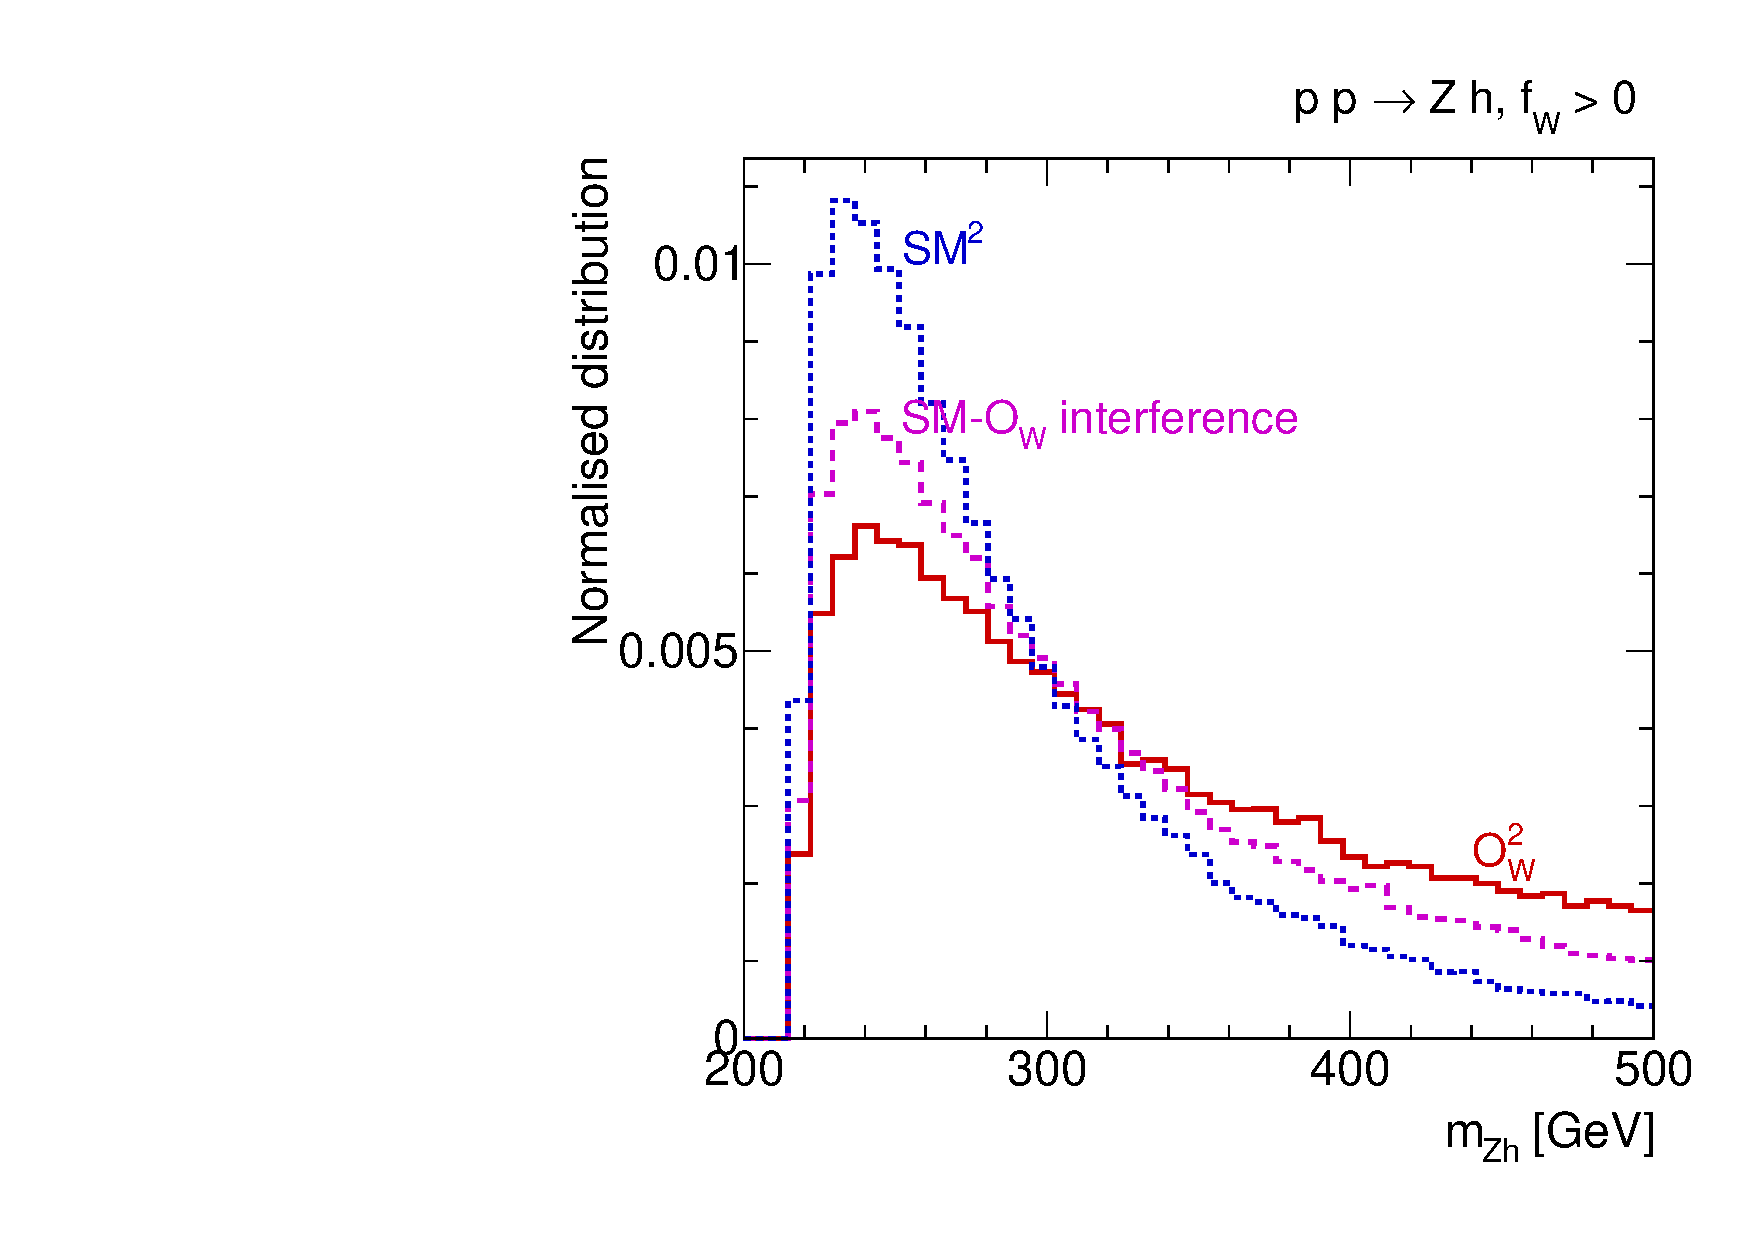
\includegraphics[width=0.49\textwidth,clip=true,trim=0 0.5cm 0 0.5cm]{fig/general/dim6demo1.pdf}
  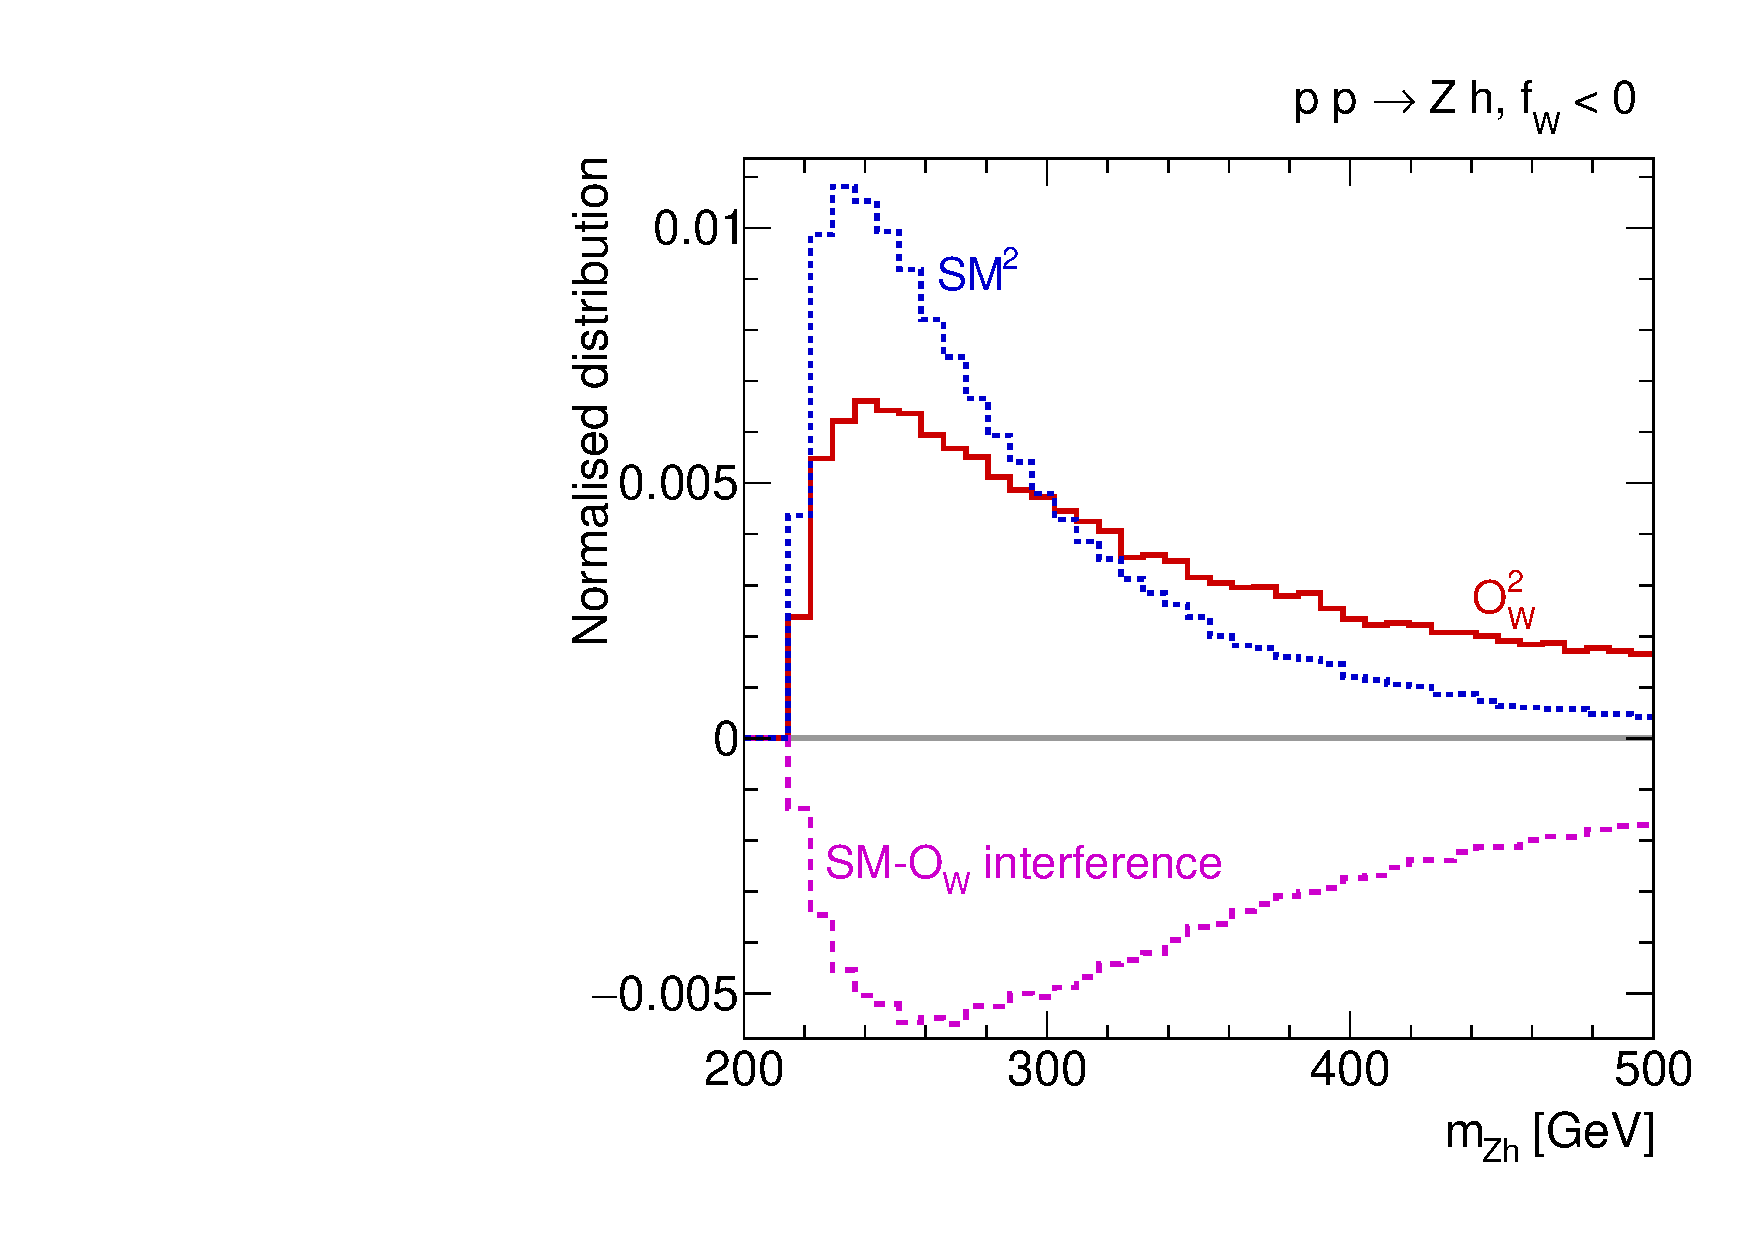
\includegraphics[width=0.49\textwidth,clip=true,trim=0 0.5cm 0 0.5cm]{fig/general/dim6demo2.pdf}
  \caption[Momentum dependence from $\ope{W}$ in $Zh$
  production]{Distribution of the $Zh$ invariant mass in the
    Higgs-strahlung process $pp \to Zh$ at LHC conditions at
    $\sqrt{s} = 13~\tev$. We compare the SM contributions to the
    squared amplitude from the operator $\ope{W}$ and to their
    interference.  Depending on the sign of the Wilson coefficient
    $f_W$, the latter can be constructive (left) or destructive
    (right).}
    % Note that this plot is based on a different
    % operator basis, which is why the operator $\ope{W}$ used in this
    % plot is closely related, but not identical to that defined in
    % \autoref{tbl:foundations_operators_bosonic_even}.
  \label{fig:foundations_OW_Zh_demo}
\end{figure}

This operator illustrates two key features of the EFT approach. First,
$\ope{W}$ does not only affect the $hWW$ vertex, but also $hZZ$
interactions and triple-gauge couplings such as $WWZ$. This means that
the dimension-six operator language allows us to combine different
measurements in a global fit.

Second, $\ope{W}$ changes the shape of distributions, for instance in
Higgs-strahlung at the LHC,
%
\begin{equation}
  p p \to Z h \,.
\end{equation}
%
In this process, the intermediate $Z$ can carry arbitrarily large
energy and momentum, which we can measure for instance as the
invariant mass of the final $Zh$ system. From
\autoref{eq:foundations_OW_HWW_Feynman_rule} we expect the effect from
$\ope{W}$ to grow with $m_{Zh}$. In
\autoref{fig:foundations_OW_Zh_demo} we demonstrate this by comparing
the distribution of $m_{Zh}$ based on the SM diagrams alone with the
squared amplitudes from the dimension-six operator $\ope{W}$ and the
interference between the two components. Indeed we see that $\ope{W}$
contributes mostly in the high-energy tail of the distribution.




%%%%%%%%%%%%%%%%%%%%%%%%%%%%%%%%%%%%%%%%%%%%%%%%%%%%%%%%%%%%
\subsubsection{All those couplings}
%%%%%%%%%%%%%%%%%%%%%%%%%%%%%%%%%%%%%%%%%%%%%%%%%%%%%%%%%%%%

After these two worked-out examples, we now give the complete list of
single-Higgs couplings induced by the dimension-six operators of
Equations~\eqref{eq:foundations_operators_even} and
\eqref{eq:foundations_operators_odd}~\cite{Corbett:2012ja,
  Juan_thesis, Tyler_thesis}.\footnote{When comparing with
  References~\cite{Corbett:2012ja, Juan_thesis, Tyler_thesis}, note
  the different sign conventions in the covariant derivative.}

These interactions read
%
\begin{align}
  \lgr{EFT} &\supset
              g^{(1)}_{hgg} \; h G^a_{\mu\nu} G^{a \, \mu\nu}
              + g^{(2)}_{hgg} \; \varepsilon_{\mu \nu \rho \sigma} h G^{a\, \mu\nu} G^{a \, \rho\sigma}
              + g^{\vphantom{(1)}}_{h\gamma\gamma} \; h A_{\mu \nu} A^{\mu \nu} \notag \\
            &\phantom{{}={}}
              + g^{(1)}_{hZ\gamma} \; A_{\mu \nu} Z^{\mu} \partial^{\nu} h
              + g^{(2)}_{hZ\gamma} \; h A_{\mu \nu} Z^{\mu \nu} \notag \\
            &\phantom{{}={}}
              + g^{(1)}_{hZZ}  \; Z_{\mu \nu} Z^{\mu} \partial^{\nu} h
              + g^{(2)}_{hZZ}  \; h Z_{\mu \nu} Z^{\mu \nu}
              + g^{(3)}_{hZZ}  \; h Z_\mu Z^\mu 
              + g^{(4)}_{hZZ}  \; h \varepsilon_{\mu \nu \rho \sigma}  Z^{\mu \nu} Z^{\rho \sigma} \notag \\
            &\phantom{{}={}}
              + g^{(1)}_{hWW}  \; \left (W^+_{\mu \nu} W^{- \, \mu} \partial^{\nu} h + \hc \right)
              + g^{(2)}_{hWW}  \; h W^+_{\mu \nu} W^{- \, \mu \nu}
              + g^{(3)}_{hWW}  \; h W^+_{\mu} W^{- \, \mu} \notag \\
            &\phantom{{}={}}
              + g^{(4)}_{hWW}  \; h \varepsilon_{\mu \nu \rho \sigma} W^{+ \, \mu \nu} W^{- \, \rho \sigma}
              + \sum_{f=\tau,t,b} \left( g^{\vphantom{(1)}}_{hff} \; h \overbar{f}_L f_R + \hc \right) 
  \label{eq:foundations_higgs_interactions}
\end{align}
%
with couplings
%
\begingroup%
\allowdisplaybreaks%
\begin{align}
  g^{(1)}_{hgg} &= \frac {f_{GG} v} {\Lambda^2} \left(1 +  \frac{v^2  f_{\phi,2} } {\Lambda^2} \right)^{-1/2} \,, \notag \\
  %
  g^{(2)}_{hgg} &= \frac {f_{G\widetilde{G}} v} {2 \Lambda^2} \left(1 +  \frac{v^2  f_{\phi,2} } {\Lambda^2} \right)^{-1/2} \,, \notag \\
  %
  g^{\vphantom{(1)}}_{h\gamma\gamma} &= - \frac {g^2 v s_W^2 (f_{WW} + f_{BB}) } {4 \Lambda^2} \left(1 +  \frac{v^2  f_{\phi,2} } {\Lambda^2} \right)^{-1/2} \,, \notag \\
  %
  g^{(1)}_{hZ\gamma}  &= - \frac {g^2 v s_W (f_{W} - f_{B}) } {4 c_W \Lambda^2} \left(1 +  \frac{v^2  f_{\phi,2} } {\Lambda^2} \right)^{-1/2}\,, \notag \\
  %
  g^{(2)}_{hZ\gamma} &= \frac {g^2 v s_W (2 s_W^2 f_{BB} - 2 c_W^2 f_{WW}) } {4 c_W \Lambda^2} \left(1 +  \frac{v^2  f_{\phi,2} } {\Lambda^2} \right)^{-1/2} \,, \notag \\
  %
  g^{(1)}_{hZZ} &= - \frac {g^2 v (c_W^2 f_{W} + s_W^2 f_{B}) } {4 c_W^2 \Lambda^2} \left(1 +  \frac{v^2  f_{\phi,2} } {\Lambda^2} \right)^{-1/2} \,, \notag \\
  %
  g^{(2)}_{hZZ} &= - \frac {g^2 v (s_W^4 f_{BB} + c_W^4 f_{WW}) } {4 c_W^2 \Lambda^2} \left(1 +  \frac{v^2  f_{\phi,2} } {\Lambda^2} \right)^{-1/2} \,, \notag \\
  %
  g^{(3)}_{hZZ} &= \frac {g^2 v} {4 c_W^2} \left(1 +  \frac{v^2  f_{\phi,2} } {\Lambda^2} \right)^{-1/2} \,, \notag \\
  g^{(4)}_{hZZ} &= - \frac {g^2 v (s_W^4 f_{B\widetilde{B}} + c_W^4 f_{W\widetilde{W}}) } {8 c_W^2 \Lambda^2} \left(1 +  \frac{v^2  f_{\phi,2} } {\Lambda^2} \right)^{-1/2} \,, \notag \\
  %
  g^{(1)}_{hWW} &= - \frac {g^2 v f_W } {4 \Lambda^2} \left(1 +  \frac{v^2  f_{\phi,2} } {\Lambda^2} \right)^{-1/2} \,, \notag \\
  g^{(2)}_{hWW} &= - \frac {g^2 v f_{WW}} {2 \Lambda^2} \left(1 +  \frac{v^2  f_{\phi,2} } {\Lambda^2} \right)^{-1/2} \,, \notag \\
  g^{(3)}_{hWW} &= \frac {g^2 v} {2} \left(1 +  \frac{v^2  f_{\phi,2} } {\Lambda^2} \right)^{-1/2}  \,, \notag \\
  %
  g^{(4)}_{hWW} &= - \frac {g^2 v f_{W\widetilde{W}}} {4 \Lambda^2}  \left(1 +  \frac{v^2  f_{\phi,2} } {\Lambda^2} \right)^{-1/2} \,, \qquad \text{and} \notag \\
  %
  g^{\vphantom{(1)}}_{hff} &= - \frac {m_f} {v} \left(1 +  \frac{v^2  f_{\phi,2} } {\Lambda^2} \right)^{-1/2}
  + \frac {v^2 f_f} {\sqrt{2} \Lambda^2} \,.
  \label{eq:foundations_higgs_couplings}
\end{align}%
\endgroup
%
Here $s_W = g' / \sqrt{g^2 + g'^2}$ and $c_W = g / \sqrt{g^2 + g'^2}$
are the sine and cosine of the weak mixing angle, and
$V_{\mu\nu} = \partial_\mu V_\nu - \partial_\nu V_\mu$ for
$V = A, W^\pm, Z$.

Note that the clear majority of the couplings in
\autoref{eq:foundations_higgs_interactions} does not exist in the SM
and contains derivatives. Dimension-six operators predict a variety of
novel kinematic features in Higgs interactions, making their
measurement at the LHC both exciting and challenging.



%%%%%%%%%%%%%%%%%%%%%%%%%%%%%%%%%%%%%%%%%%%%%%%%%%%%%%%%%%%%
\subsection{Alternative frameworks}
\label{sec:foundations_heft_alternatives}
%%%%%%%%%%%%%%%%%%%%%%%%%%%%%%%%%%%%%%%%%%%%%%%%%%%%%%%%%%%%

The linear Higgs EFT discussed above is not the only useful
parametrisation of Higgs properties. We briefly go through some
of the alternative frameworks and explain their main properties,
before concluding this chapter with a comparison between the different
approaches.



%%%%%%%%%%%%%%%%%%%%%%%%%%%%%%%%%%%%%%%%%%%%%%%%%%%%%%%%%%%%
\subsubsection{Non-linear Higgs effective field theory}
%%%%%%%%%%%%%%%%%%%%%%%%%%%%%%%%%%%%%%%%%%%%%%%%%%%%%%%%%%%%

In the SM EFT (or linear Higgs EFT), constructed in
\autoref{sec:foundations_heft_operators}, the Higgs boson $h$ and the
Goldstone bosons $w^a$ form an $SU(2)_L$ doublet $\phi$ as given in
\autoref{eq:foundations_sm_phi}. But in some models of new physics the
Higgs\footnote{In many scenarios of new physics the observed scalar at
  $125~\gev$ is, of course, not the Higgs boson of the Standard
  Model. We nevertheless refer to it as `Higgs boson'.} is not part of
an elementary doublet. Typical examples are composite Higgs models in
which the Higgs boson is a pseudo-Goldstone from some strongly
interacting dynamics~\cite{Kaplan:1983fs, Kaplan:1983sm, Banks:1984gj,
  Agashe:2004rs, Gripaios:2009pe}. Non-linear Higgs EFT, sometimes
simply called `Higgs EFT', is an effective theory designed for these
scenarios~\cite{Appelquist:1980vg, Longhitano:1980iz,
  Appelquist:1984rr, Grinstein:2007iv, Alonso:2012px,
  Buchalla:2013rka, Buchalla:2013eza, Brivio:2013pma, Gavela:2014vra,
  Buchalla:2015wfa, Brivio:2016fzo}. This model is also often referred
to as `chiral Lagrangian', and indeed its structure is similar to that
of chiral perturbation theory, for an introduction see for instance
References~\cite{Scherer:2002tk, HillerBlin:2016jpb}.  Again, we begin
by going through the ingredients to the effective theory before
constructing the Lagrangian.

The \emph{particle content} of the non-linear Higgs EFT constitutes
the main difference to the linear Lagrangian: the physical scalar $h$
is separated from the Goldstones $w^a$, both are included as
independent degrees of freedom rather than as part of the doublet
$\phi$. The Higgs boson $h$ is now a singlet under the SM gauge
symmetry.  The Goldstone bosons $w^a$ are organised in the exponential
form
% 
\begin{equation}
  U = e^{\im \sigma^a w^a/v} \,,
\end{equation}
% 
where $\sigma^a$ are the Pauli matrices.
The Goldstones transform non-linearly under the (approximate) global
custodial symmetry $SU(2)_L \times SU(2)_R$, giving the EFT its name.

The \emph{symmetries} are the same as in the linear case. We require
invariance under Lorentz transformations as well as under the SM gauge
group $SU(3)_C \times SU(2)_L \times U(1)_Y$ and baryon and lepton
number conservation. For simplicity, we also focus our brief
discussion on $CP$-even operators that conserve lepton flavour.

Choosing the \emph{counting scheme} is a little more complex. To
account for strongly interacting scenarios, we now have to distinguish
three different scales~\cite{Buchalla:2013eza}:
% 
\begin{itemize}
\item the electroweak scale $v = 246~\gev$, which defines the $W$ and
  $Z$ mass, but is not necessarily the Higgs VEV;
  % 
\item the scale $f$ associated to the Goldstone bosons $w^a$ and the
  Higgs boson $h$ due to some breaking of the underlying
  dynamics\footnote{In general, the scales associated with $w^a$ and
    $h$, $f_w$ and $f_h$, can be different, making the power-counting
    even more complicated.}, in analogy to the pion decay constant
  $f_\pi$; and
  % 
\item the cut-off $\Lambda$ of the theory. For weakly coupled physics
  its value is arbitrary. But it can be calculated that the low-energy
  effective theories from spontaneously broken strongly coupled
  dynamics break down around
  $\Lambda \approx 4 \pi f$~\cite{Scherer:2002tk}. A cut-off of this
  size guarantees that the EFT is renormalisable order by order.
\end{itemize}

The existence of three scales means there are two dimensionless
parameters, so in general the EFT terms are organised in a double
expansion~\cite{Buchalla:2013eza}. The first is
% 
\begin{equation}
  \xi \equiv \frac {v^2} {f^2} \,.
\end{equation}
% 
The value of $\xi$ defines the non-linearity of the model: the limit
$\xi \to 0$ restores the linear Lagrangian. An expansion in $\xi$
exactly corresponds to the power-counting scheme of the linear EFT,
i.\,e.\ it orders operators by their canonical dimension.

The second dimensionless parameter is
% 
\begin{equation}
  \frac {f^2} {\Lambda^2} \approx \frac 1 {16 \pi^2}
\end{equation}
% 
for strongly coupled scenarios. Since this is of the same size as a
loop factor, expanding in $f^2/\Lambda^2$ corresponds to a loop
expansion, similar to that in chiral perturbation theory. Equivalently,
one can define a \emph{chiral dimension} $\chi = [\ope{}]_c$ for each
operator $\ope{}$ with the assignments~\cite{Buchalla:2013eza}
% 
\begin{align}
  [f]_c &= 1 \,, \quad &
  [A_{\mu}]_c &= 0 \,, \quad & 
  [F_{\mu\nu}]_c &= 1 \,, \quad &
  [U]_c &= 0 \,, \quad &
  [h]_c &= 0 \,, \quad \notag \\
  [\partial_\mu]_c &= 1 \,, \quad  &
  [D_\mu]_c &= 1 \,, \quad &
  [g]_c &= 1 \,, \quad &
  [y_f]_c &= 1 \,,
\end{align}
%
where we use $A_\mu$ and $F_{\mu\nu}$ to denote any vector boson,
since the symbol $V_\mu$ is conventionally used for a different
purpose in this context. The loop order $L$ of an operator is
equivalent to the chiral dimension $\chi = 2L + 2$. This chiral
counting can also be linked to an expansion in
$\hbar$~\cite{Gavela:2016bzc}.

The correct expansion scheme depends on the value of $\xi$. For
$\xi \gg 1 / 16 \pi^2$ or $f \ll 3~\tev$, the chiral expansion is more
appropriate. For $\xi \ll 1 / 16 \pi^2$ or $f \gg 3~\tev$, the
canonical expansion is correct. In the intermediate region, a combined
expansion gives the best results. Since LHC Higgs physics is mostly
sensitive to new physics scenarios with $f \ll 3~\tev$, the chiral expansion
can be considered phenomenologically more relevant. For a more
thorough discussion of power counting in this framework, see
Reference~\cite{Krause:2016uhw}.

\newparagraph
%
At the leading chiral order $\chi = 2$ or $L = 0$, the Higgs sector of
the Lagrangian is given by~\cite{Alonso:2012px}\footnote{Two comments
  on this Lagrangian are in order. First, in principle there could be
  further functions of $h$ coupling to the kinetic terms of the gauge
  bosons. Such interactions arise in typical strongly coupled theories
  at one-loop level with a coefficient $\sim 1 / (16 \pi^2)$ and are
  therefore usually classified as NLO operators~\cite{Alonso:2012px,
    Buchalla:2013rka}. Second, the function $\mathcal{F}_C(h)$ (and a
  corresponding one for the fermion kinetic terms) can be removed with
  field redefinitions, shifting its effects into the other
  couplings~\cite{Buchalla:2013rka, Brivio:2016fzo}.}
%
\begin{align}
  \lgr{non-linear EFT}
  &\supset \frac 1 2 \, \partial_\mu h \, \partial^\mu h \, \left( 1 + c_H \xi \, \mathcal{F}_H(h) \right)
    - V(h) \notag \\
  &\phantom{{}={}} - \frac {v^2} 4 \, \tr [ V_\mu V^\mu] \, \mathcal{F}_C(h) 
    + c_T \xi \frac {v^2} 4 \, \tr [T V^\mu] \tr [T V_\mu] \, \mathcal{F}_T(h) \notag \\
  &\phantom{{}={}} - \frac v {\sqrt{2}} \, \left[ \sum_f \overbar{f}_L \, U \, y_f \, \mathcal{F}_Y^{f}(h) \, P_f \, f_R + \hc \right]
  \label{eq:foundations_nonlinear_EFT_LO}
\end{align}
%
with $V_\mu \equiv (D_\mu U) U^\dagger$,
$T \equiv U \sigma_3 U^\dagger$ and projectors
$P_u = (\mathds{1} + \sigma_3) / 2$,
$P_d = P_\ell = (\mathds{1} - \sigma_3)/2$.  The functions
$\mathcal{F}_C(h)$, $V(h)$, $\mathcal{F}_T(h)$, $\mathcal{F}_T(h)$,
$\mathcal{F}_Y^{u}(h)$, $\mathcal{F}_Y^{d}(h)$, and
$\mathcal{F}_Y^{\ell}(h)$ encode the coupling of the Higgs $h$ and are
arbitrary functions. They can be expanded as a power series in $h/f$,
or to simplify the expressions in $h/v$, for instance
%
\begin{equation}
  \mathcal{F}_C(h) = 1 + 2a_C \, \frac h v + b_C \, \left(\frac h v \right)^2 + \dots \,.
\end{equation}

At next-to-leading order in the chiral expansion, many more terms
relevant for Higgs physics appear. We do not list them here and refer
the interested reader for example to Reference~\cite{Brivio:2013pma}.

\newparagraph
%
Finally, the relationship between the linear and non-linear effective
theories deserves some discussion. The two approaches in principle
provide different parametrisations of the same physics, as can be
seen by expanding the non-linear Lagrangian in $\xi$ rather than
$\chi$. The difference is the ordering of the operators in the EFT
expansion and, equivalently, the expected size of different
effects. Operators that appear at one order in the $1/\Lambda$
expansion of the linear EFT may appear at a very different order in
the chiral expansion of the non-linear EFT.

Since the symmetry requirements on the non-linear setup are smaller,
we expect it to be more general than the linear Lagrangian at a
comparable order in the expansions. This is exactly what is found when
comparing the linear dimension-six operators to the NLO chiral
Lagrangian: the dimension-six operators predict certain correlations,
while the non-linear description has more operators that can break
these correlations~\cite{Brivio:2013pma}. A straightforward example is
the relation between $hxx$ and $hhxx$ couplings. For dimension-six
operators of the form $\phisq x x$, this ratio is fixed to $2v$, since
$\phisq \sim (v^2 + 2vh + h^2) / 2$. In the chiral approach, these
couplings are always independent, as can be seen in
\autoref{eq:foundations_nonlinear_EFT_LO}.

The current experimental limits leave room for both strongly or weakly
coupled new physics, for $\xi$ smaller or larger than
$1 / (16 \pi^2)$, for scenarios in which the linear or non-linear
effective theories work better. Only a precise measurement of the
Higgs properties and a global analysis of correlations will tell us
which approach is correct. As a general rule, more SM-like results
favour the linear approach that we follow throughout this
thesis~\cite{Krause:2016uhw}. On the other hand, certain deviations
that do not follow the correlations predicted by dimension-six
operators point towards non-linear physics~\cite{Brivio:2013pma}.



%%%%%%%%%%%%%%%%%%%%%%%%%%%%%%%%%%%%%%%%%%%%%%%%%%%%%%%%%%%%
\subsubsection{$\kappa$ framework}
%%%%%%%%%%%%%%%%%%%%%%%%%%%%%%%%%%%%%%%%%%%%%%%%%%%%%%%%%%%%

Effective field theories are of course not the only way to describe
the Higgs sector. During Run~1 of the LHC, the most widely used
parametrisation was the $\kappa$
framework~\cite{LHCHiggsCrossSectionWorkingGroup:2012nn} or the
closely related $\Delta$ framework~\cite{Lafaye:2009vr}. Its
construction is remarkably simple: starting from the SM Higgs sector,
all Higgs couplings are dressed with form factors,
%
\begin{equation}
  g_{hxx} = \kappa_{\vphantom{h}x}^{\vphantom{\text{SM}}} \, g_{hxx}^{\text{SM}} \equiv \left(1 + \Delta_{\vphantom{h}x}^{\vphantom{\text{SM}}} \right) \, g_{hxx}^{\text{SM}} \,,
  \label{eq:foundations_kappa_delta}
\end{equation}
%
such that $\kappa_x = 1$ or $\Delta_x = 0$ corresponds to the SM
couplings.  Some care has to be taken to treat the Higgs-gluon and
Higgs-photon couplings consistently, where indirect effects of shifted
Higgs-top or Higgs-$W$ couplings compete with direct effects from new
physics~\cite{Lafaye:2009vr}.

From a theoretical point of view, the $\kappa$ framework is not
gauge-invariant and does not present a consistent quantum field
theory. In particular, calculating electroweak loop effects in the
$\kappa$ framework can introduce divergences that cannot be
renormalised~\cite{Passarino:2012cb}. This problem can be solved by
embedding the $\kappa$ framework in a UV
completion~\cite{Lopez-Val:2013yba}.

From a more phenomenological point of view, this approach is well
suited to parametrise measurements of total rates. Simple shifts of
SM-like Higgs coupling structures are expected in some scenarios of
new physics, for instance in many scalar extensions of the Higgs
sector~\cite{Lopez-Val:2013yba}. But many other models predict new
kinematic features, visible as changed kinematic shapes, and the
$\kappa$ framework is unable to describe these. For better or worse,
it is also agnostic about correlations between different Higgs
couplings, and about correlations between Higgs observables and triple
gauge vertices or electroweak precision measurements.

The strength of the $\kappa$ framework is clearly not its theoretical
foundation. Its allure comes from its simplicity and the fact that it
is designed around the simple question of measuring the couplings of
the (SM-like) Higgs boson. This parametrisation made sense as a
common denominator for the first Higgs measurements with limited
statistics of Run~1 of the LHC. But the increased amount of data and
crucial kinematic information collected during Run~2 require a
different, more sophisticated language.



%%%%%%%%%%%%%%%%%%%%%%%%%%%%%%%%%%%%%%%%%%%%%%%%%%%%%%%%%%%%
\subsubsection{Pseudo-Observables}
%%%%%%%%%%%%%%%%%%%%%%%%%%%%%%%%%%%%%%%%%%%%%%%%%%%%%%%%%%%%

Higgs pseudo-observables (POs)~\cite{Isidori:2013cga, Bordone:2015nqa,
  Greljo:2015sla} are designed as a generalisation of the $\kappa$
framework to include BSM kinematic features. In a very broad sense,
this term encompasses any quantity that is field theoretically defined
and can be experimentally accessed~\cite{Krause:2016uhw}. Signal
strengths, cross sections, partial widths, total widths, and
individual form factors or couplings all fall under this umbrella
term. Here we follow the more narrow definition of effective-coupling
POs~\cite{deFlorian:2016spz}. They are defined process by process by
writing down all contributing amplitudes under some broad assumptions
on new physics. These expressions are then decomposed in a pole
expansion, and the resulting residues are identified as
pseudo-observables. This procedure also requires an expansion in the
inverse of the new physics scale $\Lambda$. Just as the EFT approach,
pseudo-observables thus rely on new physics being heavy,
$E \ll \Lambda$. So far, this framework has been developed for Higgs
production in WBF and Higgs-strahlung, as well as for all
phenomenologically relevant Higgs decays.

Phenomenologically, pseudo-observables can describe shifts in SM
couplings as well as kinematic shapes. Like the EFT approach, their
construction requires certain minimal assumptions on the symmetries of
new physics as well as an expansion in $1/\Lambda$. In fact, at tree
level pseudo-observables can be mapped directly to the Wilson
coefficients of an EFT constructed with the same ingredients (which is
the non-linear Higgs EFT discussed above).

The main difference between pseudo-observables and the EFT approach is
a conceptual one. Pseudo-observables are designed from the perspective
of a given process: they describe the coefficients of the different
contributing amplitudes. They are not parameters of a Lagrangian and
do not define a consistent quantum field theory. In particular, the
values of POs measured in one process have no meaning for other
processes. Effective operators on the other hand are a proper,
gauge-invariant quantum field theory that universally describes any
physics below the cutoff scale, and the same Wilson coefficients
predict the behaviour of very different processes.

Proponents of the PO approach favour a multi-layer interpretation of
LHC data, where the data is first presented in terms of
pseudo-observables, and can then be interpreted in terms of EFTs or
specific models of UV physics. They argue that this approach provides
a clear separation between measurement and
interpretation~\cite{deFlorian:2016spz}. On the other hand, proponents
of the `direct EFT approach' argue that there is no need for such an
intermediate layer, and suggest to directly fit effective
operators. The debate about which approach is better is still
ongoing~\cite{deFlorian:2016spz}. Ultimately, both effective operators
and POs are well-defined frameworks that can describe all relevant
kinematic effects, and thus present a suitable interface between
experiment and theory.



%%%%%%%%%%%%%%%%%%%%%%%%%%%%%%%%%%%%%%%%%%%%%%%%%%%%%%%%%%%%
\subsubsection{Simplified models}
%%%%%%%%%%%%%%%%%%%%%%%%%%%%%%%%%%%%%%%%%%%%%%%%%%%%%%%%%%%%

The parametrisations discussed so far have in common that they assume
the absence of new light particles. Simplified models are designed to
close this gap and to describe kinematic effects from new light
resonances. In addition to resonance peaks, these include threshold
effects in loops and Higgs decays into (invisible) new light degrees
of freedom. Simplified models thus allow to combine information from
direct searches with indirect measurements. Except for the key element
of adding new light propagating degrees of freedom to the SM, the term
is not particularly well-defined, and there is a lot of freedom to
construct such models.

The simplest version of a simplified model consists of the SM
supplemented with another particle, with ad-hoc coupling structures
based on phenomenological requirements~\cite{Biekotter:2016ecg}. Such
a setup might even be not gauge-invariant and thus inconsistent beyond
tree level. At the other end of the spectrum, simplified models can be
consistently defined quantum field theories, potentially involving
higher-dimensional operators. The only difference to the linear and
non-linear EFT approaches discussed above is the extended particle
content. The additional flexibility, of course, comes at the price of an
increased number of parameters.

Examples of such models for Higgs physics include an extended Higgs
sector with an additional singlet and a doublet, which offers great
flexibility to tune the Higgs couplings~\cite{Lopez-Val:2013yba}. The
authors of Reference~\cite{Dolan:2016eki} develop a model with an
additional singlet and vector-like quarks. Finally,
References~\cite{Gripaios:2016xuo, Bauer:2016hcu} discuss additional
scalar singlets supplemented with higher-dimensional operators.



%%%%%%%%%%%%%%%%%%%%%%%%%%%%%%%%%%%%%%%%%%%%%%%%%%%%%%%%%%%%
\subsubsection{Comparison}
%%%%%%%%%%%%%%%%%%%%%%%%%%%%%%%%%%%%%%%%%%%%%%%%%%%%%%%%%%%%

\begin{table}
  \renewcommand{\arraystretch}{1.8}
  \footnotesize
  \begin{tabularx}{\textwidth}{LLLLLL} 
    \toprule 
    %
    & $\kappa$ framework & POs & Non-linear EFT & Linear EFT & Simplified models \\
    \midrule
    %
    Motivation & 
    experiment: \newline simplest Higgs parametrisation &
    experiment: \newline amplitude decomposition for a given process &
    theory: \newline complete low-energy effects of NP with singlet $h$& 
    theory: \newline complete low-energy effects of NP with doublet $\phi$ &
    exp.\,/\,theory:\newline new light particles \\
    %
    Input & 
    SM Higgs couplings &
    process amplitudes, \newline pole expansion,  \newline NP expansion ($1/\Lambda $)&
    SM particles ($h$), \newline symmetries, \newline counting scheme (loops) & 
    SM particles ($\phi$), \newline symmetries, \newline counting scheme ($1/\Lambda $) & 
    new particles (masses, charges, interactions) \\
    %
    Parameters & 
    coefficients of SM amplitude &
    coefficients of SM \& NP amplitudes &
    Lagrangian parameters of consistent QFT & 
    Lagrangian parameters of consistent QFT &
    depends \\
    %
    Validity conditions & 
    SM-like NP &
    NP heavy, symmetries &
    NP heavy, symmetries & 
    NP heavy, symmetries &
    single light new particles, other NP decouples \\
    \midrule 
    %
    Shifted SM couplings & 
    yes &
    yes &
    yes & 
    yes &
    depends \\
    %
    Kinematic effects & 
    no &
    yes &
    yes & 
    yes &
    depends \\
    %
    New resonances, \newline loop thresholds, \newline invisible decays & 
    no &
    no &
    no & 
    no &
    yes \\
    %
    Correlations & 
    no &
    no &
    some & 
    many &
    depends \\
    % \midrule
    % %
    % WBF parameters &
    % $\kappa_W$
    % &
    % $\kappa_{WW}$, $\varepsilon_{WW}$, $\varepsilon_{WW}^{CP}$, $\varepsilon_{Wu_L}$ &
    % &
    % $\frac {f_{\phi,2}} {\Lambda^2}$, $\frac {f_{W}} {\Lambda^2}$, $\frac {f_{WW}} {\Lambda^2}$, $\frac {f_{W\widetilde{W}}} {\Lambda^2}$ & 
    % depends \\
    %                                                                                                
    \bottomrule
  \end{tabularx}
  \caption[Comparison between different parametrisations of Higgs properties]{Comparison
    between different parametrisations of Higgs properties. The upper part of the table
    focuses on the theoretical foundation, the lower on the phenomenology.
% Finally, we list some parameters relevant for WBF Higgs
% production in the different approaches, restricting this example to
% the dominant $W$-mediated amplitude.
    Since `simplified models' describe a rather general idea, many
    details depend on the specific realisation.}
  \label{tbl:foundations_framework_comparison}
\end{table}

All of these approaches define parametrisations of the Higgs properties
that can be used as interfaces between different measurements and
between experiment and theory. In
\autoref{tbl:foundations_framework_comparison} we summarise and
compare their different properties.

The different frameworks can be classified into consistent quantum
field theories, which include the EFTs, and process-based
parametrisations of amplitudes through form factors, such as the
$\kappa$ framework and pseudo-observables. Simplified models can fall
into either category. Only the QFT formalism allows to link different
processes and to incorporate any loop effects.

More important for practical purposes is the range of phenomena that
can be described. The $\kappa$ framework is limited to rescalings of
the SM Higgs couplings and is not able to incorporate kinematic
information. Pseudo-observables and the two EFT approaches are much
more flexible and can describe a large number of kinematic
features. However, they rely on new physics being substantially
heavier than the experimentally probed energies around the weak
scale. Features from light new particles, for instance resonances or
loop thresholds, are only covered by appropriate simplified
models. The dimension-six operators of linear Higgs EFT, and to a
lesser extent the leading operators of the chiral EFT, also predict
certain correlations between different couplings and measurements,
whereas by definition the pseudo-observables are only valid for a given
process.

To summarise, in the absence of new light particles, Higgs properties
can be adequately parametrised by pseudo-observables, non-linear Higgs
EFT, and linear Higgs EFT. The linear EFT approach is theoretically
consistent, well-motivated, and phenomenologically powerful, and we
focus on this framework during this thesis.



% Maybe the simplest model of new physics is the extension of the SM by one real scalar singlet, also known as a `Higgs portal'. This new field $s$ only couples to the Higgs doublet $\phi$ proportional to its mass $m_s$ times a coupling $\lambda_s$. Identifying $\Lambda = m_s$ and integrating out the singlet gives rise to the diagram
% \begin{align}
%   \raisebox{-0.5\height}{
%     %\fbox{
%       \fmfframe(0,5)(-1,5){ %(L,T) (R,B)
%         \begin{fmfgraph*}(35,20)
%           \fmfleft{i2,i1}
%           \fmfright{o2,o1}
%           \fmflabel{$\phi^\dagger$}{i1}
%           \fmflabel{$\phi$}{i2}
%           \fmflabel{$\phi^\dagger$}{o1}
%           \fmflabel{$\phi$}{o2}
%           \fmf{dashes}{i1,v1,i2}
%           \fmf{dashes}{o1,v2,o2}
%           \fmf{dbl_dashes,tension=1,label=$s$}{v1,v2}
%           \marrow{m}{up}{top}{$p$}{v1,v2}
%         \end{fmfgraph*}
%       }
%     %}
%   }
%   &\sim (\phisq) \frac {m_s^2 \lambda_s^2}{p^2 - m_s^2} (\phisq) \notag \\
%   {} &\sim  \lambda_s^2  (\phisq) \left(1 + \frac {p^2} {\Lambda^2} + \ord{1/\Lambda^4}\right) (\phisq) \notag \\
%   {} &\sim  \lambda_s^2  (\phisq) \left(1 - \frac {\partial^2} {\Lambda^2} + \ord{1/m_s^4}\right) (\phisq) \\
%   {} &\sim  \lambda_s^2  (\phisq)^2 + \frac {\lambda_s^2} {\Lambda^2} \, \partial_\mu (\phisq) \partial^\mu (\phisq) \,.
% \end{align}

% The first term is an unobservable renormalisation of an SM operator, but the second one is just $\ope{\phi2}$ with Wilson coefficient $f_{\phi,2} = 2\lambda_s^2$. At tree level, this is the only operator generated by this model.